\PassOptionsToPackage{unicode=true}{hyperref} % options for packages loaded elsewhere
\PassOptionsToPackage{hyphens}{url}
%
\documentclass[]{article}
\usepackage{lmodern}
\usepackage{amssymb,amsmath}
\usepackage{ifxetex,ifluatex}
\usepackage{fixltx2e} % provides \textsubscript
\ifnum 0\ifxetex 1\fi\ifluatex 1\fi=0 % if pdftex
  \usepackage[T1]{fontenc}
  \usepackage[utf8]{inputenc}
  \usepackage{textcomp} % provides euro and other symbols
\else % if luatex or xelatex
  \usepackage{unicode-math}
  \defaultfontfeatures{Ligatures=TeX,Scale=MatchLowercase}
\fi
% use upquote if available, for straight quotes in verbatim environments
\IfFileExists{upquote.sty}{\usepackage{upquote}}{}
% use microtype if available
\IfFileExists{microtype.sty}{%
\usepackage[]{microtype}
\UseMicrotypeSet[protrusion]{basicmath} % disable protrusion for tt fonts
}{}
\IfFileExists{parskip.sty}{%
\usepackage{parskip}
}{% else
\setlength{\parindent}{0pt}
\setlength{\parskip}{6pt plus 2pt minus 1pt}
}
\usepackage{hyperref}
\hypersetup{
            pdftitle={JACC study Milk intake and stroke mortality analysis},
            pdfauthor={Chaochen Wang},
            pdfborder={0 0 0},
            breaklinks=true}
\urlstyle{same}  % don't use monospace font for urls
\usepackage[margin=1in]{geometry}
\usepackage{color}
\usepackage{fancyvrb}
\newcommand{\VerbBar}{|}
\newcommand{\VERB}{\Verb[commandchars=\\\{\}]}
\DefineVerbatimEnvironment{Highlighting}{Verbatim}{commandchars=\\\{\}}
% Add ',fontsize=\small' for more characters per line
\usepackage{framed}
\definecolor{shadecolor}{RGB}{248,248,248}
\newenvironment{Shaded}{\begin{snugshade}}{\end{snugshade}}
\newcommand{\AlertTok}[1]{\textcolor[rgb]{0.94,0.16,0.16}{#1}}
\newcommand{\AnnotationTok}[1]{\textcolor[rgb]{0.56,0.35,0.01}{\textbf{\textit{#1}}}}
\newcommand{\AttributeTok}[1]{\textcolor[rgb]{0.77,0.63,0.00}{#1}}
\newcommand{\BaseNTok}[1]{\textcolor[rgb]{0.00,0.00,0.81}{#1}}
\newcommand{\BuiltInTok}[1]{#1}
\newcommand{\CharTok}[1]{\textcolor[rgb]{0.31,0.60,0.02}{#1}}
\newcommand{\CommentTok}[1]{\textcolor[rgb]{0.56,0.35,0.01}{\textit{#1}}}
\newcommand{\CommentVarTok}[1]{\textcolor[rgb]{0.56,0.35,0.01}{\textbf{\textit{#1}}}}
\newcommand{\ConstantTok}[1]{\textcolor[rgb]{0.00,0.00,0.00}{#1}}
\newcommand{\ControlFlowTok}[1]{\textcolor[rgb]{0.13,0.29,0.53}{\textbf{#1}}}
\newcommand{\DataTypeTok}[1]{\textcolor[rgb]{0.13,0.29,0.53}{#1}}
\newcommand{\DecValTok}[1]{\textcolor[rgb]{0.00,0.00,0.81}{#1}}
\newcommand{\DocumentationTok}[1]{\textcolor[rgb]{0.56,0.35,0.01}{\textbf{\textit{#1}}}}
\newcommand{\ErrorTok}[1]{\textcolor[rgb]{0.64,0.00,0.00}{\textbf{#1}}}
\newcommand{\ExtensionTok}[1]{#1}
\newcommand{\FloatTok}[1]{\textcolor[rgb]{0.00,0.00,0.81}{#1}}
\newcommand{\FunctionTok}[1]{\textcolor[rgb]{0.00,0.00,0.00}{#1}}
\newcommand{\ImportTok}[1]{#1}
\newcommand{\InformationTok}[1]{\textcolor[rgb]{0.56,0.35,0.01}{\textbf{\textit{#1}}}}
\newcommand{\KeywordTok}[1]{\textcolor[rgb]{0.13,0.29,0.53}{\textbf{#1}}}
\newcommand{\NormalTok}[1]{#1}
\newcommand{\OperatorTok}[1]{\textcolor[rgb]{0.81,0.36,0.00}{\textbf{#1}}}
\newcommand{\OtherTok}[1]{\textcolor[rgb]{0.56,0.35,0.01}{#1}}
\newcommand{\PreprocessorTok}[1]{\textcolor[rgb]{0.56,0.35,0.01}{\textit{#1}}}
\newcommand{\RegionMarkerTok}[1]{#1}
\newcommand{\SpecialCharTok}[1]{\textcolor[rgb]{0.00,0.00,0.00}{#1}}
\newcommand{\SpecialStringTok}[1]{\textcolor[rgb]{0.31,0.60,0.02}{#1}}
\newcommand{\StringTok}[1]{\textcolor[rgb]{0.31,0.60,0.02}{#1}}
\newcommand{\VariableTok}[1]{\textcolor[rgb]{0.00,0.00,0.00}{#1}}
\newcommand{\VerbatimStringTok}[1]{\textcolor[rgb]{0.31,0.60,0.02}{#1}}
\newcommand{\WarningTok}[1]{\textcolor[rgb]{0.56,0.35,0.01}{\textbf{\textit{#1}}}}
\usepackage{graphicx,grffile}
\makeatletter
\def\maxwidth{\ifdim\Gin@nat@width>\linewidth\linewidth\else\Gin@nat@width\fi}
\def\maxheight{\ifdim\Gin@nat@height>\textheight\textheight\else\Gin@nat@height\fi}
\makeatother
% Scale images if necessary, so that they will not overflow the page
% margins by default, and it is still possible to overwrite the defaults
% using explicit options in \includegraphics[width, height, ...]{}
\setkeys{Gin}{width=\maxwidth,height=\maxheight,keepaspectratio}
\setlength{\emergencystretch}{3em}  % prevent overfull lines
\providecommand{\tightlist}{%
  \setlength{\itemsep}{0pt}\setlength{\parskip}{0pt}}
\setcounter{secnumdepth}{5}
% Redefines (sub)paragraphs to behave more like sections
\ifx\paragraph\undefined\else
\let\oldparagraph\paragraph
\renewcommand{\paragraph}[1]{\oldparagraph{#1}\mbox{}}
\fi
\ifx\subparagraph\undefined\else
\let\oldsubparagraph\subparagraph
\renewcommand{\subparagraph}[1]{\oldsubparagraph{#1}\mbox{}}
\fi

% set default figure placement to htbp
\makeatletter
\def\fps@figure{htbp}
\makeatother

\usepackage{bookmark}
\usepackage{xltxtra}
\usepackage{zxjatype}
\usepackage[ipaex]{zxjafont}

\title{JACC study Milk intake and stroke mortality analysis}
\author{Chaochen Wang}
\date{2019-12-20 created, 2020-01-09 updated}

\begin{document}
\maketitle

{
\setcounter{tocdepth}{3}
\tableofcontents
}
\hypertarget{read-in-the-data}{%
\section{Read in the data}\label{read-in-the-data}}

\begin{Shaded}
\begin{Highlighting}[]
\KeywordTok{library}\NormalTok{(readr)}
\KeywordTok{library}\NormalTok{(tidyverse)}
\end{Highlighting}
\end{Shaded}

\begin{verbatim}
## -- Attaching packages ------------------------------------------------------------------------------------------------ tidyverse 1.3.0 --
\end{verbatim}

\begin{verbatim}
## v ggplot2 3.2.1     v dplyr   0.8.3
## v tibble  2.1.3     v stringr 1.4.0
## v tidyr   1.0.0     v forcats 0.4.0
## v purrr   0.3.3
\end{verbatim}

\begin{verbatim}
## -- Conflicts --------------------------------------------------------------------------------------------------- tidyverse_conflicts() --
## x dplyr::filter() masks stats::filter()
## x dplyr::lag()    masks stats::lag()
\end{verbatim}

\begin{Shaded}
\begin{Highlighting}[]
\KeywordTok{library}\NormalTok{(lubridate) }\CommentTok{# for dealing with date time data }
\end{Highlighting}
\end{Shaded}

\begin{verbatim}
## 
## Attaching package: 'lubridate'
\end{verbatim}

\begin{verbatim}
## The following object is masked from 'package:base':
## 
##     date
\end{verbatim}

\begin{Shaded}
\begin{Highlighting}[]
\NormalTok{MILK <-}\StringTok{ }\KeywordTok{read_csv}\NormalTok{(}\StringTok{"../data/StrokeMilk.csv"}\NormalTok{, }
                     \DataTypeTok{progress =} \KeywordTok{show_progress}\NormalTok{(), }
                     \DataTypeTok{col_types =} \KeywordTok{cols}\NormalTok{(}\DataTypeTok{.default =} \StringTok{"c"}\NormalTok{))}

\NormalTok{MILK }\OperatorTok\StringTok{ }
\StringTok{  }\KeywordTok{filter}\NormalTok{(tr_age }\OperatorTok{>}\StringTok{ }\DecValTok{39} \OperatorTok{&}\StringTok{ }\NormalTok{tr_age }\OperatorTok{<}\StringTok{ }\DecValTok{80}\NormalTok{) }\OperatorTok\StringTok{ }
\StringTok{  }\KeywordTok{group_by}\NormalTok{(tr_sex) }\OperatorTok\StringTok{ }
\StringTok{  }\KeywordTok{summarise}\NormalTok{(}\DataTypeTok{n=} \KeywordTok{n}\NormalTok{()) }\OperatorTok
\StringTok{  }\KeywordTok{mutate}\NormalTok{(}\DataTypeTok{rel.freq =} \KeywordTok{paste0}\NormalTok{(}\KeywordTok{round}\NormalTok{(}\DecValTok{100} \OperatorTok{*}\StringTok{ }\NormalTok{n}\OperatorTok{/}\KeywordTok{sum}\NormalTok{(n), }\DecValTok{2}\NormalTok{), }\StringTok{"%"}\NormalTok{))  }
\end{Highlighting}
\end{Shaded}

\begin{verbatim}
## # A tibble: 2 x 3
##   tr_sex     n rel.freq
##   <chr>  <int> <chr>   
## 1 1      46395 41.95%  
## 2 2      64190 58.05%
\end{verbatim}

\hypertarget{delete-subjects-outside-of-age-range}{%
\section{delete subjects outside of age range
------------------------------------}\label{delete-subjects-outside-of-age-range}}

\begin{Shaded}
\begin{Highlighting}[]
\NormalTok{MILK_}\DecValTok{0}\NormalTok{ <-}\StringTok{ }\NormalTok{MILK }\OperatorTok
\StringTok{  }\KeywordTok{filter}\NormalTok{(tr_age }\OperatorTok{>}\StringTok{ }\DecValTok{39} \OperatorTok{&}\StringTok{ }\NormalTok{tr_age }\OperatorTok{<}\StringTok{ }\DecValTok{80}\NormalTok{)}
\end{Highlighting}
\end{Shaded}

\hypertarget{define-total-stroke-mortality}{%
\section{define total stroke mortality
--------------------------------}\label{define-total-stroke-mortality}}

\begin{Shaded}
\begin{Highlighting}[]
\NormalTok{MILK_}\DecValTok{0}\NormalTok{ <-}\StringTok{ }\NormalTok{MILK_}\DecValTok{0} \OperatorTok\StringTok{ }
\StringTok{  }\KeywordTok{mutate}\NormalTok{(}\DataTypeTok{Tot_Stroke =} \KeywordTok{if_else}\NormalTok{(}\KeywordTok{grepl}\NormalTok{(}\StringTok{"I6[0-9][0-9]|I6[0-9]"}\NormalTok{,  }
\NormalTok{                                    ICD10), }\StringTok{"I60_9"}\NormalTok{, }
                        \KeywordTok{if_else}\NormalTok{(}\OperatorTok{!}\KeywordTok{is.na}\NormalTok{(ICD10), }\StringTok{"other_death"}\NormalTok{, }
                                      \StringTok{"Alive/Censor"}\NormalTok{))) }
\NormalTok{MILK_}\DecValTok{0}\OperatorTok\StringTok{ }
\StringTok{  }\KeywordTok{group_by}\NormalTok{(tr_sex, Tot_Stroke) }\OperatorTok
\StringTok{  }\KeywordTok{summarise}\NormalTok{(}\DataTypeTok{n=} \KeywordTok{n}\NormalTok{()) }\OperatorTok
\StringTok{  }\KeywordTok{mutate}\NormalTok{(}\DataTypeTok{rel.freq =} \KeywordTok{paste0}\NormalTok{(}\KeywordTok{round}\NormalTok{(}\DecValTok{100} \OperatorTok{*}\StringTok{ }\NormalTok{n}\OperatorTok{/}\KeywordTok{sum}\NormalTok{(n), }\DecValTok{2}\NormalTok{), }\StringTok{"%"}\NormalTok{))}
\end{Highlighting}
\end{Shaded}

\begin{verbatim}
## # A tibble: 6 x 4
## # Groups:   tr_sex [2]
##   tr_sex Tot_Stroke       n rel.freq
##   <chr>  <chr>        <int> <chr>   
## 1 1      Alive/Censor 31110 67.05%  
## 2 1      I60_9         1825 3.93%   
## 3 1      other_death  13460 29.01%  
## 4 2      Alive/Censor 52347 81.55%  
## 5 2      I60_9         1777 2.77%   
## 6 2      other_death  10066 15.68%
\end{verbatim}

\hypertarget{define-different-type-of-stroke-mortalitycvd}{%
\section{define different type of stroke mortality/CVD
?---------------------------}\label{define-different-type-of-stroke-mortalitycvd}}

I60 Nontraumatic subarachnoid hemorrhage

I61 Nontraumatic intracerebral hemorrhage

I62 Other and unspecified nontraumatic intracranial hemorrhage

I63 Cerebral infarction

I65 Occlusion and stenosis of precerebral arteries, not resulting in
cerebral infarction

I66 Occlusion and stenosis of cerebral arteries, not resulting in
cerebral infarction

I67 Other cerebrovascular diseases

I68 Cerebrovascular disorders in diseases classified elsewhere

I69 Sequelae of cerebrovascular disease

\begin{Shaded}
\begin{Highlighting}[]
\NormalTok{MILK_}\DecValTok{0}\NormalTok{ <-}\StringTok{ }\NormalTok{MILK_}\DecValTok{0} \OperatorTok\StringTok{ }
\StringTok{  }\KeywordTok{mutate}\NormalTok{(}\DataTypeTok{HemoStroke =} \KeywordTok{if_else}\NormalTok{(}\KeywordTok{grepl}\NormalTok{(}\StringTok{"I6[0-2][0-9]|I6[0-2]"}\NormalTok{,  }
\NormalTok{                                    ICD10), }\StringTok{"I60_2"}\NormalTok{, }
                              \KeywordTok{if_else}\NormalTok{(}\OperatorTok{!}\KeywordTok{is.na}\NormalTok{(ICD10), }\StringTok{"other_death"}\NormalTok{, }
                                      \StringTok{"Alive/Censor"}\NormalTok{))) }\OperatorTok\StringTok{ }
\StringTok{  }\KeywordTok{mutate}\NormalTok{(}\DataTypeTok{IscheStroke =} \KeywordTok{if_else}\NormalTok{(}\KeywordTok{grepl}\NormalTok{(}\StringTok{"I63[0-9]|I63"}\NormalTok{,  }
\NormalTok{                                    ICD10), }\StringTok{"I63"}\NormalTok{, }
                              \KeywordTok{if_else}\NormalTok{(}\OperatorTok{!}\KeywordTok{is.na}\NormalTok{(ICD10), }\StringTok{"other_death"}\NormalTok{, }
                                      \StringTok{"Alive/Censor"}\NormalTok{))) }\OperatorTok
\StringTok{  }\KeywordTok{mutate}\NormalTok{(}\DataTypeTok{CHD =} \KeywordTok{if_else}\NormalTok{(}\KeywordTok{grepl}\NormalTok{(}\StringTok{"I2[0-5][0-9]|I2[0-5]"}\NormalTok{,  }
\NormalTok{                                     ICD10), }\StringTok{"I20_5"}\NormalTok{, }
                               \KeywordTok{if_else}\NormalTok{(}\OperatorTok{!}\KeywordTok{is.na}\NormalTok{(ICD10), }\StringTok{"other_death"}\NormalTok{, }
                                       \StringTok{"Alive/Censor"}\NormalTok{))) }\OperatorTok
\StringTok{  }\KeywordTok{mutate}\NormalTok{(}\DataTypeTok{HeartF =} \KeywordTok{if_else}\NormalTok{(}\KeywordTok{grepl}\NormalTok{(}\StringTok{"I50[0-9]|I50"}\NormalTok{,  }
\NormalTok{                                     ICD10), }\StringTok{"I50"}\NormalTok{, }
                               \KeywordTok{if_else}\NormalTok{(}\OperatorTok{!}\KeywordTok{is.na}\NormalTok{(ICD10), }\StringTok{"other_death"}\NormalTok{, }
                                       \StringTok{"Alive/Censor"}\NormalTok{)))}


\NormalTok{MILK_}\DecValTok{0}\OperatorTok\StringTok{ }
\StringTok{  }\KeywordTok{group_by}\NormalTok{(tr_sex, HemoStroke) }\OperatorTok
\StringTok{  }\KeywordTok{summarise}\NormalTok{(}\DataTypeTok{n=} \KeywordTok{n}\NormalTok{()) }\OperatorTok
\StringTok{  }\KeywordTok{mutate}\NormalTok{(}\DataTypeTok{rel.freq =} \KeywordTok{paste0}\NormalTok{(}\KeywordTok{round}\NormalTok{(}\DecValTok{100} \OperatorTok{*}\StringTok{ }\NormalTok{n}\OperatorTok{/}\KeywordTok{sum}\NormalTok{(n), }\DecValTok{2}\NormalTok{), }\StringTok{"%"}\NormalTok{))}
\end{Highlighting}
\end{Shaded}

\begin{verbatim}
## # A tibble: 6 x 4
## # Groups:   tr_sex [2]
##   tr_sex HemoStroke       n rel.freq
##   <chr>  <chr>        <int> <chr>   
## 1 1      Alive/Censor 31110 67.05%  
## 2 1      I60_2          556 1.2%    
## 3 1      other_death  14729 31.75%  
## 4 2      Alive/Censor 52347 81.55%  
## 5 2      I60_2          666 1.04%   
## 6 2      other_death  11177 17.41%
\end{verbatim}

\begin{Shaded}
\begin{Highlighting}[]
\NormalTok{MILK_}\DecValTok{0}\OperatorTok\StringTok{ }
\StringTok{  }\KeywordTok{group_by}\NormalTok{(tr_sex, IscheStroke) }\OperatorTok
\StringTok{  }\KeywordTok{summarise}\NormalTok{(}\DataTypeTok{n=} \KeywordTok{n}\NormalTok{()) }\OperatorTok
\StringTok{  }\KeywordTok{mutate}\NormalTok{(}\DataTypeTok{rel.freq =} \KeywordTok{paste0}\NormalTok{(}\KeywordTok{round}\NormalTok{(}\DecValTok{100} \OperatorTok{*}\StringTok{ }\NormalTok{n}\OperatorTok{/}\KeywordTok{sum}\NormalTok{(n), }\DecValTok{2}\NormalTok{), }\StringTok{"%"}\NormalTok{))}
\end{Highlighting}
\end{Shaded}

\begin{verbatim}
## # A tibble: 6 x 4
## # Groups:   tr_sex [2]
##   tr_sex IscheStroke      n rel.freq
##   <chr>  <chr>        <int> <chr>   
## 1 1      Alive/Censor 31110 67.05%  
## 2 1      I63            705 1.52%   
## 3 1      other_death  14580 31.43%  
## 4 2      Alive/Censor 52347 81.55%  
## 5 2      I63            600 0.93%   
## 6 2      other_death  11243 17.52%
\end{verbatim}

\begin{Shaded}
\begin{Highlighting}[]
\NormalTok{MILK_}\DecValTok{0}\OperatorTok\StringTok{ }
\StringTok{  }\KeywordTok{group_by}\NormalTok{(tr_sex, CHD) }\OperatorTok
\StringTok{  }\KeywordTok{summarise}\NormalTok{(}\DataTypeTok{n=} \KeywordTok{n}\NormalTok{()) }\OperatorTok
\StringTok{  }\KeywordTok{mutate}\NormalTok{(}\DataTypeTok{rel.freq =} \KeywordTok{paste0}\NormalTok{(}\KeywordTok{round}\NormalTok{(}\DecValTok{100} \OperatorTok{*}\StringTok{ }\NormalTok{n}\OperatorTok{/}\KeywordTok{sum}\NormalTok{(n), }\DecValTok{2}\NormalTok{), }\StringTok{"%"}\NormalTok{))}
\end{Highlighting}
\end{Shaded}

\begin{verbatim}
## # A tibble: 6 x 4
## # Groups:   tr_sex [2]
##   tr_sex CHD              n rel.freq
##   <chr>  <chr>        <int> <chr>   
## 1 1      Alive/Censor 31110 67.05%  
## 2 1      I20_5         1003 2.16%   
## 3 1      other_death  14282 30.78%  
## 4 2      Alive/Censor 52347 81.55%  
## 5 2      I20_5          758 1.18%   
## 6 2      other_death  11085 17.27%
\end{verbatim}

\begin{Shaded}
\begin{Highlighting}[]
\NormalTok{MILK_}\DecValTok{0}\OperatorTok\StringTok{ }
\StringTok{  }\KeywordTok{group_by}\NormalTok{(tr_sex, HeartF) }\OperatorTok
\StringTok{  }\KeywordTok{summarise}\NormalTok{(}\DataTypeTok{n=} \KeywordTok{n}\NormalTok{()) }\OperatorTok
\StringTok{  }\KeywordTok{mutate}\NormalTok{(}\DataTypeTok{rel.freq =} \KeywordTok{paste0}\NormalTok{(}\KeywordTok{round}\NormalTok{(}\DecValTok{100} \OperatorTok{*}\StringTok{ }\NormalTok{n}\OperatorTok{/}\KeywordTok{sum}\NormalTok{(n), }\DecValTok{2}\NormalTok{), }\StringTok{"%"}\NormalTok{))}
\end{Highlighting}
\end{Shaded}

\begin{verbatim}
## # A tibble: 6 x 4
## # Groups:   tr_sex [2]
##   tr_sex HeartF           n rel.freq
##   <chr>  <chr>        <int> <chr>   
## 1 1      Alive/Censor 31110 67.05%  
## 2 1      I50            711 1.53%   
## 3 1      other_death  14574 31.41%  
## 4 2      Alive/Censor 52347 81.55%  
## 5 2      I50            799 1.24%   
## 6 2      other_death  11044 17.21%
\end{verbatim}

\hypertarget{define-milk-intake}{%
\section{Define milk intake
---------------------------------------------}\label{define-milk-intake}}

\begin{Shaded}
\begin{Highlighting}[]
\NormalTok{MILK_}\DecValTok{0}\NormalTok{ <-}\StringTok{ }\NormalTok{MILK_}\DecValTok{0} \OperatorTok\StringTok{ }
\StringTok{  }\KeywordTok{mutate}\NormalTok{(}\DataTypeTok{Milk_fre =} \KeywordTok{as.numeric}\NormalTok{(MILK)) }\OperatorTok\StringTok{ }
\StringTok{  }\KeywordTok{mutate}\NormalTok{(}\DataTypeTok{Milk_fre =} \KeywordTok{as.factor}\NormalTok{(Milk_fre)) }\OperatorTok\StringTok{ }
\StringTok{  }\KeywordTok{mutate}\NormalTok{(}\DataTypeTok{Mlkfre =} \KeywordTok{fct_collapse}\NormalTok{(Milk_fre,}
                               \DataTypeTok{Never =} \StringTok{"1"}\NormalTok{,}
                               \DataTypeTok{Mon1_2 =} \StringTok{"2"}\NormalTok{, }
                               \DataTypeTok{Wek1_2 =} \StringTok{"3"}\NormalTok{,}
                               \DataTypeTok{Wek3_4 =} \StringTok{"4"}\NormalTok{,}
                               \DataTypeTok{Daily  =} \StringTok{"5"}\NormalTok{)) }\OperatorTok\StringTok{ }
\StringTok{  }\KeywordTok{mutate}\NormalTok{(}\DataTypeTok{MlkLogi =} \KeywordTok{fct_collapse}\NormalTok{(Mlkfre,}
                                \DataTypeTok{Never =} \StringTok{"Never"}\NormalTok{, }
                                \DataTypeTok{Drinker =} \KeywordTok{c}\NormalTok{(}\StringTok{"Mon1_2"}\NormalTok{, }\StringTok{"Wek1_2"}\NormalTok{, }\StringTok{"Wek3_4"}\NormalTok{, }\StringTok{"Daily"}\NormalTok{)))}
\end{Highlighting}
\end{Shaded}

\begin{verbatim}
## Warning: NAs introduced by coercion
\end{verbatim}

\begin{Shaded}
\begin{Highlighting}[]
\NormalTok{MILK_}\DecValTok{0} \OperatorTok\StringTok{ }
\StringTok{  }\KeywordTok{group_by}\NormalTok{(tr_sex, Mlkfre) }\OperatorTok
\StringTok{  }\KeywordTok{summarise}\NormalTok{(}\DataTypeTok{n=} \KeywordTok{n}\NormalTok{()) }\OperatorTok
\StringTok{  }\KeywordTok{mutate}\NormalTok{(}\DataTypeTok{rel.freq =} \KeywordTok{paste0}\NormalTok{(}\KeywordTok{round}\NormalTok{(}\DecValTok{100} \OperatorTok{*}\StringTok{ }\NormalTok{n}\OperatorTok{/}\KeywordTok{sum}\NormalTok{(n), }\DecValTok{2}\NormalTok{), }\StringTok{"%"}\NormalTok{))}
\end{Highlighting}
\end{Shaded}

\begin{verbatim}
## Warning: Factor `Mlkfre` contains implicit NA, consider using
## `forcats::fct_explicit_na`
\end{verbatim}

\begin{verbatim}
## # A tibble: 12 x 4
## # Groups:   tr_sex [2]
##    tr_sex Mlkfre     n rel.freq
##    <chr>  <fct>  <int> <chr>   
##  1 1      Never   8961 19.31%  
##  2 1      Mon1_2  3691 7.96%   
##  3 1      Wek1_2  6228 13.42%  
##  4 1      Wek3_4  5862 12.63%  
##  5 1      Daily  17110 36.88%  
##  6 1      <NA>    4543 9.79%   
##  7 2      Never  10960 17.07%  
##  8 2      Mon1_2  3830 5.97%   
##  9 2      Wek1_2  7975 12.42%  
## 10 2      Wek3_4  8516 13.27%  
## 11 2      Daily  26957 42%     
## 12 2      <NA>    5952 9.27%
\end{verbatim}

\begin{Shaded}
\begin{Highlighting}[]
\NormalTok{MILK_}\DecValTok{0} \OperatorTok\StringTok{ }
\StringTok{  }\KeywordTok{group_by}\NormalTok{(tr_sex, MlkLogi) }\OperatorTok
\StringTok{  }\KeywordTok{summarise}\NormalTok{(}\DataTypeTok{n=} \KeywordTok{n}\NormalTok{()) }\OperatorTok
\StringTok{  }\KeywordTok{mutate}\NormalTok{(}\DataTypeTok{rel.freq =} \KeywordTok{paste0}\NormalTok{(}\KeywordTok{round}\NormalTok{(}\DecValTok{100} \OperatorTok{*}\StringTok{ }\NormalTok{n}\OperatorTok{/}\KeywordTok{sum}\NormalTok{(n), }\DecValTok{2}\NormalTok{), }\StringTok{"%"}\NormalTok{))}
\end{Highlighting}
\end{Shaded}

\begin{verbatim}
## Warning: Factor `MlkLogi` contains implicit NA, consider using
## `forcats::fct_explicit_na`
\end{verbatim}

\begin{verbatim}
## # A tibble: 6 x 4
## # Groups:   tr_sex [2]
##   tr_sex MlkLogi     n rel.freq
##   <chr>  <fct>   <int> <chr>   
## 1 1      Never    8961 19.31%  
## 2 1      Drinker 32891 70.89%  
## 3 1      <NA>     4543 9.79%   
## 4 2      Never   10960 17.07%  
## 5 2      Drinker 47278 73.65%  
## 6 2      <NA>     5952 9.27%
\end{verbatim}

\hypertarget{calculate-person-years}{%
\section{Calculate person-years}\label{calculate-person-years}}

\begin{Shaded}
\begin{Highlighting}[]
\NormalTok{MILK_}\DecValTok{0}\NormalTok{ <-}\StringTok{ }\NormalTok{MILK_}\DecValTok{0} \OperatorTok\StringTok{ }
\StringTok{  }\KeywordTok{mutate}\NormalTok{(}\DataTypeTok{Age =} \KeywordTok{as.numeric}\NormalTok{(tr_age)) }\OperatorTok\StringTok{ }
\StringTok{  }\KeywordTok{mutate}\NormalTok{(}\DataTypeTok{followpy =} \KeywordTok{as.numeric}\NormalTok{(actual)}\OperatorTok{/}\FloatTok{365.25}\NormalTok{) }
\end{Highlighting}
\end{Shaded}

\hypertarget{identify-potential-confounders-smoking-alcohol-intake-bmi-dmhytmiapocancer-history-exercise-energy-intake-sleep-duration-vegetablefrugreteacofe-intake-school-education}{%
\section{Identify potential confounders: smoking, alcohol intake, BMI,
DM/HYT/MI/APO/Cancer history, Exercise, Energy intake, Sleep duration,
vegetable/fru/gretea/cofe intake, school
education}\label{identify-potential-confounders-smoking-alcohol-intake-bmi-dmhytmiapocancer-history-exercise-energy-intake-sleep-duration-vegetablefrugreteacofe-intake-school-education}}

\begin{Shaded}
\begin{Highlighting}[]
\NormalTok{MILK_}\DecValTok{0}\NormalTok{ <-}\StringTok{  }\NormalTok{MILK_}\DecValTok{0} \OperatorTok\StringTok{ }
\StringTok{  }\KeywordTok{mutate}\NormalTok{(}\DataTypeTok{Smoking =} \KeywordTok{replace_na}\NormalTok{(SM1, }\StringTok{"unknown"}\NormalTok{)) }\OperatorTok\StringTok{ }
\StringTok{  }\KeywordTok{mutate}\NormalTok{(}\DataTypeTok{Smoking =} \KeywordTok{as_factor}\NormalTok{(Smoking)) }\OperatorTok\StringTok{ }
\StringTok{  }\KeywordTok{mutate}\NormalTok{(}\DataTypeTok{Smoking =} \KeywordTok{fct_recode}\NormalTok{(Smoking, }\DataTypeTok{Never =} \StringTok{"3"}\NormalTok{, }\DataTypeTok{Past =} \StringTok{"2"}\NormalTok{, }\DataTypeTok{Current =} \StringTok{"1"}\NormalTok{)) }\OperatorTok\StringTok{ }
\StringTok{  }\KeywordTok{mutate}\NormalTok{(}\DataTypeTok{Smoking =} \KeywordTok{factor}\NormalTok{(Smoking, }\DataTypeTok{levels =} \KeywordTok{c}\NormalTok{(}\StringTok{"Never"}\NormalTok{, }\StringTok{"Past"}\NormalTok{, }\StringTok{"Current"}\NormalTok{, }\StringTok{"unknown"}\NormalTok{))) }\OperatorTok\StringTok{  }\CommentTok{# Smoking}
\StringTok{  }\KeywordTok{mutate}\NormalTok{(}\DataTypeTok{Alc_Fre =} \KeywordTok{if_else}\NormalTok{(}\KeywordTok{as.numeric}\NormalTok{(DR1) }\OperatorTok{>=}\StringTok{ }\DecValTok{2}\NormalTok{, }\StringTok{"Never or past"}\NormalTok{, }
                           \KeywordTok{if_else}\NormalTok{(}\KeywordTok{as.numeric}\NormalTok{(DR1F) }\OperatorTok{==}\StringTok{ }\DecValTok{1}\NormalTok{, }\StringTok{"Daily"}\NormalTok{, }
                                   \KeywordTok{if_else}\NormalTok{(}\KeywordTok{as.numeric}\NormalTok{(DR1F) }\OperatorTok{==}\StringTok{ }\DecValTok{4}\NormalTok{, }\StringTok{"< 1/week"}\NormalTok{, }
                                           \KeywordTok{if_else}\NormalTok{((}\KeywordTok{as.numeric}\NormalTok{(DR1F) }\OperatorTok{==}\StringTok{ }\DecValTok{2}\NormalTok{) }\OperatorTok{|}\StringTok{ }\NormalTok{(}\KeywordTok{as.numeric}\NormalTok{(DR1F) }\OperatorTok{==}\StringTok{ }\DecValTok{3}\NormalTok{), }
                                                   \StringTok{"1-4 /week"}\NormalTok{, }\StringTok{"Unknown"}\NormalTok{))))) }\OperatorTok\StringTok{ }
\StringTok{  }\KeywordTok{mutate}\NormalTok{(}\DataTypeTok{Alc_Fre =} \KeywordTok{fct_explicit_na}\NormalTok{(Alc_Fre, }\DataTypeTok{na_level =} \StringTok{"unknown"}\NormalTok{)) }\OperatorTok\StringTok{ }
\StringTok{  }\KeywordTok{mutate}\NormalTok{(}\DataTypeTok{BMI =} \KeywordTok{as.numeric}\NormalTok{(wt10)}\OperatorTok{/}\NormalTok{(}\KeywordTok{as.numeric}\NormalTok{(ht10)}\OperatorTok{^}\DecValTok{2}\NormalTok{) }\OperatorTok{*}\StringTok{ }\DecValTok{100000}\NormalTok{) }\OperatorTok\StringTok{ }\CommentTok{# define BMI groups}
\StringTok{  }\KeywordTok{mutate}\NormalTok{(}\DataTypeTok{BMIgrp =} \KeywordTok{cut}\NormalTok{(BMI, }\DataTypeTok{breaks =} \KeywordTok{c}\NormalTok{(}\DecValTok{14}\NormalTok{, }\FloatTok{18.5}\NormalTok{, }\DecValTok{25}\NormalTok{, }\DecValTok{30}\NormalTok{, }\DecValTok{40}\NormalTok{), }\DataTypeTok{right =} \OtherTok{FALSE}\NormalTok{)) }\OperatorTok\StringTok{ }
\StringTok{  }\KeywordTok{mutate}\NormalTok{(}\DataTypeTok{BMIgrp =} \KeywordTok{as.character}\NormalTok{(BMIgrp)) }\OperatorTok\StringTok{ }
\StringTok{  }\KeywordTok{replace_na}\NormalTok{(}\KeywordTok{list}\NormalTok{(}\DataTypeTok{BMIgrp =} \StringTok{"unknown"}\NormalTok{)) }\OperatorTok\StringTok{ }
\StringTok{  }\KeywordTok{mutate}\NormalTok{(}\DataTypeTok{BMIgrp =} \KeywordTok{factor}\NormalTok{(BMIgrp, }\DataTypeTok{levels =} \KeywordTok{c}\NormalTok{(}\StringTok{"[18.5,25)"}\NormalTok{,}
                                            \StringTok{"[14,18.5)"}\NormalTok{,}
                                            \StringTok{"[25,30)"}\NormalTok{, }
                                            \StringTok{"[30,40)"}\NormalTok{, }\StringTok{"unknown"}\NormalTok{))) }\OperatorTok
\StringTok{  }\KeywordTok{mutate}\NormalTok{(}\DataTypeTok{DM_hist =} \KeywordTok{if_else}\NormalTok{(}\KeywordTok{as.numeric}\NormalTok{(p_DM) }\OperatorTok{>}\StringTok{ }\DecValTok{1}\NormalTok{, }\OtherTok{TRUE}\NormalTok{, }\OtherTok{FALSE}\NormalTok{)) }\OperatorTok\StringTok{ }
\StringTok{  }\KeywordTok{replace_na}\NormalTok{(}\KeywordTok{list}\NormalTok{(}\DataTypeTok{DM_hist =} \StringTok{"unknown"}\NormalTok{)) }\OperatorTok\StringTok{ }\CommentTok{# recode DM history status}
\StringTok{  }\KeywordTok{mutate}\NormalTok{(}\DataTypeTok{HT_hist =} \KeywordTok{if_else}\NormalTok{(}\KeywordTok{as.numeric}\NormalTok{(p_HT) }\OperatorTok{>}\StringTok{ }\DecValTok{1}\NormalTok{, }\OtherTok{TRUE}\NormalTok{, }\OtherTok{FALSE}\NormalTok{)) }\OperatorTok\StringTok{ }
\StringTok{  }\KeywordTok{replace_na}\NormalTok{(}\KeywordTok{list}\NormalTok{(}\DataTypeTok{HT_hist =} \StringTok{"unknown"}\NormalTok{)) }\OperatorTok\StringTok{ }\CommentTok{# recode hyt history status}
\StringTok{  }\KeywordTok{mutate}\NormalTok{(}\DataTypeTok{MI_hist =} \KeywordTok{if_else}\NormalTok{(}\KeywordTok{as.numeric}\NormalTok{(p_MI) }\OperatorTok{>}\StringTok{ }\DecValTok{1}\NormalTok{, }\OtherTok{TRUE}\NormalTok{, }\OtherTok{FALSE}\NormalTok{)) }\OperatorTok\StringTok{ }
\StringTok{  }\KeywordTok{replace_na}\NormalTok{(}\KeywordTok{list}\NormalTok{(}\DataTypeTok{MI_hist =} \StringTok{"unknown"}\NormalTok{)) }\OperatorTok\StringTok{ }\CommentTok{# recode MI history status}
\StringTok{  }\KeywordTok{mutate}\NormalTok{(}\DataTypeTok{APO_hist =} \KeywordTok{if_else}\NormalTok{(}\KeywordTok{as.numeric}\NormalTok{(p_APO) }\OperatorTok{>}\StringTok{ }\DecValTok{1}\NormalTok{, }\OtherTok{TRUE}\NormalTok{, }\OtherTok{FALSE}\NormalTok{)) }\OperatorTok\StringTok{ }
\StringTok{  }\KeywordTok{replace_na}\NormalTok{(}\KeywordTok{list}\NormalTok{(}\DataTypeTok{APO_hist =} \StringTok{"unknown"}\NormalTok{)) }\OperatorTok\StringTok{ }\CommentTok{# recode APO history status}
\StringTok{  }\KeywordTok{mutate}\NormalTok{(}\DataTypeTok{KID_hist =} \KeywordTok{if_else}\NormalTok{(}\KeywordTok{as.numeric}\NormalTok{(p_KID) }\OperatorTok{>}\StringTok{ }\DecValTok{1}\NormalTok{, }\OtherTok{TRUE}\NormalTok{, }\OtherTok{FALSE}\NormalTok{)) }\OperatorTok\StringTok{ }
\StringTok{  }\KeywordTok{replace_na}\NormalTok{(}\KeywordTok{list}\NormalTok{(}\DataTypeTok{KID_hist =} \StringTok{"unknown"}\NormalTok{)) }\OperatorTok\StringTok{ }\CommentTok{# recode KID history status}
\StringTok{  }\KeywordTok{mutate}\NormalTok{(}\DataTypeTok{LIV_hist =} \KeywordTok{if_else}\NormalTok{(}\KeywordTok{as.numeric}\NormalTok{(p_APO) }\OperatorTok{>}\StringTok{ }\DecValTok{1}\NormalTok{, }\OtherTok{TRUE}\NormalTok{, }\OtherTok{FALSE}\NormalTok{)) }\OperatorTok\StringTok{ }
\StringTok{  }\KeywordTok{replace_na}\NormalTok{(}\KeywordTok{list}\NormalTok{(}\DataTypeTok{LIV_hist =} \StringTok{"unknown"}\NormalTok{)) }\OperatorTok\StringTok{ }\CommentTok{# recode LIV history status}
\StringTok{  }\KeywordTok{mutate}\NormalTok{(}\DataTypeTok{Can_hist =} \KeywordTok{if_else}\NormalTok{(}\KeywordTok{as.numeric}\NormalTok{(p_can1) }\OperatorTok{>}\StringTok{ }\DecValTok{1} \OperatorTok{|}\StringTok{ }
\StringTok{                              }\KeywordTok{as.numeric}\NormalTok{(p_can2) }\OperatorTok{>}\StringTok{ }\DecValTok{1}\NormalTok{, }\OtherTok{TRUE}\NormalTok{, }\OtherTok{FALSE}\NormalTok{)) }\OperatorTok\StringTok{ }
\StringTok{  }\KeywordTok{replace_na}\NormalTok{(}\KeywordTok{list}\NormalTok{(}\DataTypeTok{Can_hist =} \StringTok{"unknown"}\NormalTok{)) }\OperatorTok\StringTok{ }\CommentTok{# recode LIV history status}
\StringTok{  }\KeywordTok{mutate}\NormalTok{(}\DataTypeTok{Exercise =} \KeywordTok{as.numeric}\NormalTok{(sport) }\OperatorTok{!=}\StringTok{ }\DecValTok{4}\NormalTok{) }\OperatorTok\StringTok{ }\CommentTok{# define exercise habits}
\StringTok{  }\KeywordTok{mutate}\NormalTok{(}\DataTypeTok{Exercise =} \KeywordTok{as.character}\NormalTok{(Exercise)) }\OperatorTok\StringTok{ }
\StringTok{  }\KeywordTok{replace_na}\NormalTok{(}\KeywordTok{list}\NormalTok{(}\DataTypeTok{Exercise =} \StringTok{"unknown"}\NormalTok{)) }\OperatorTok\StringTok{ }
\StringTok{  }\KeywordTok{mutate}\NormalTok{(}\DataTypeTok{Exercise =} \KeywordTok{factor}\NormalTok{(Exercise, }\DataTypeTok{levels =} \KeywordTok{c}\NormalTok{(}\StringTok{"FALSE"}\NormalTok{, }\StringTok{"TRUE"}\NormalTok{, }\StringTok{"unknown"}\NormalTok{))) }\OperatorTok\StringTok{ }
\StringTok{  }\KeywordTok{mutate}\NormalTok{(}\DataTypeTok{Exercise =} \KeywordTok{fct_recode}\NormalTok{(Exercise, }
                               \StringTok{"> 1h/w"}\NormalTok{ =}\StringTok{ "TRUE"}\NormalTok{, }
                               \StringTok{"Almost0"}\NormalTok{ =}\StringTok{ "FALSE"}\NormalTok{, }
                               \DataTypeTok{unknown   =} \StringTok{"unknown"}\NormalTok{)) }\OperatorTok\StringTok{ }
\StringTok{  }\KeywordTok{mutate}\NormalTok{(}\DataTypeTok{Engy =} \KeywordTok{log}\NormalTok{(}\KeywordTok{as.numeric}\NormalTok{(ENERGY))) }\OperatorTok\StringTok{ }
\StringTok{  }\KeywordTok{mutate}\NormalTok{(}\DataTypeTok{Sleep =} \KeywordTok{as.numeric}\NormalTok{(SLEEP)}\OperatorTok{/}\DecValTok{10}\NormalTok{) }\OperatorTok\StringTok{ }
\StringTok{  }\KeywordTok{mutate}\NormalTok{(}\DataTypeTok{Slepgrp =} \KeywordTok{cut}\NormalTok{(Sleep, }\DataTypeTok{breaks =} \KeywordTok{c}\NormalTok{(}\DecValTok{0}\NormalTok{, }\FloatTok{6.9}\NormalTok{, }\FloatTok{7.9}\NormalTok{, }\FloatTok{8.9}\NormalTok{, }\DecValTok{23}\NormalTok{), }\DataTypeTok{right =} \OtherTok{FALSE}\NormalTok{)) }\OperatorTok\StringTok{ }
\StringTok{  }\KeywordTok{mutate}\NormalTok{(}\DataTypeTok{Slepgrp =} \KeywordTok{as.character}\NormalTok{(Slepgrp)) }\OperatorTok\StringTok{ }
\StringTok{  }\KeywordTok{replace_na}\NormalTok{(}\KeywordTok{list}\NormalTok{(}\DataTypeTok{Slepgrp =} \StringTok{"unknown"}\NormalTok{)) }\OperatorTok\StringTok{ }
\StringTok{  }\KeywordTok{mutate}\NormalTok{(}\DataTypeTok{Slepgrp =} \KeywordTok{factor}\NormalTok{(Slepgrp, }\DataTypeTok{levels =} \KeywordTok{c}\NormalTok{(}\StringTok{"[0,6.9)"}\NormalTok{,}
                                            \StringTok{"[6.9,7.9)"}\NormalTok{,}
                                            \StringTok{"[7.9,8.9)"}\NormalTok{, }
                                            \StringTok{"[8.9,23)"}\NormalTok{, }\StringTok{"unknown"}\NormalTok{))) }\OperatorTok\StringTok{ }
\StringTok{  }\KeywordTok{mutate}\NormalTok{(}\DataTypeTok{Spi =} \KeywordTok{as.factor}\NormalTok{(SPI)) }\OperatorTok\StringTok{ }\CommentTok{# define vegetable intake}
\StringTok{  }\KeywordTok{mutate}\NormalTok{(}\DataTypeTok{Spi =} \KeywordTok{fct_collapse}\NormalTok{(Spi, }
                            \DataTypeTok{unknown =} \StringTok{"X"}\NormalTok{, }
                            \DataTypeTok{daily =} \StringTok{"5"}\NormalTok{,}
                            \DataTypeTok{Thre4tw =} \StringTok{"4"}\NormalTok{,}
                            \DataTypeTok{One2tw =} \StringTok{"3"}\NormalTok{,}
                            \DataTypeTok{Less1tm =} \KeywordTok{c}\NormalTok{(}\StringTok{"1"}\NormalTok{, }\StringTok{"2"}\NormalTok{))) }\OperatorTok\StringTok{ }
\StringTok{  }\KeywordTok{mutate}\NormalTok{(}\DataTypeTok{Spi =} \KeywordTok{fct_explicit_na}\NormalTok{(Spi, }\DataTypeTok{na_level =} \StringTok{"unknown"}\NormalTok{)) }\OperatorTok\StringTok{ }
\StringTok{  }\KeywordTok{mutate}\NormalTok{(}\DataTypeTok{Fru =} \KeywordTok{as.factor}\NormalTok{(FRU)) }\OperatorTok\StringTok{ }\CommentTok{# define fruit intake}
\StringTok{  }\KeywordTok{mutate}\NormalTok{(}\DataTypeTok{Fru =} \KeywordTok{fct_collapse}\NormalTok{(Fru, }
                            \DataTypeTok{unknown =} \StringTok{"X"}\NormalTok{,}
                            \DataTypeTok{daily =} \StringTok{"5"}\NormalTok{,}
                            \DataTypeTok{Thre4tw =} \StringTok{"4"}\NormalTok{,}
                            \DataTypeTok{One2tw =} \StringTok{"3"}\NormalTok{,}
                            \DataTypeTok{Less1tm =} \KeywordTok{c}\NormalTok{(}\StringTok{"1"}\NormalTok{, }\StringTok{"2"}\NormalTok{))) }\OperatorTok\StringTok{ }
\StringTok{  }\KeywordTok{mutate}\NormalTok{(}\DataTypeTok{Fru =} \KeywordTok{fct_explicit_na}\NormalTok{(Fru, }\DataTypeTok{na_level =} \StringTok{"unknown"}\NormalTok{)) }\OperatorTok\StringTok{ }
\StringTok{  }\KeywordTok{mutate}\NormalTok{(}\DataTypeTok{Gretea =} \KeywordTok{as.factor}\NormalTok{(GreTEA1)) }\OperatorTok\StringTok{ }\CommentTok{# define greentea intake}
\StringTok{  }\KeywordTok{mutate}\NormalTok{(}\DataTypeTok{Gretea =} \KeywordTok{fct_collapse}\NormalTok{(Gretea, }
                               \DataTypeTok{unknown =} \StringTok{"X"}\NormalTok{, }
                               \DataTypeTok{Thre3tw =} \StringTok{"2"}\NormalTok{, }
                               \DataTypeTok{Thre3tw =} \StringTok{"3"}\NormalTok{,}
                               \DataTypeTok{Thre3tw =} \StringTok{"4"}\NormalTok{,}
                               \DataTypeTok{Never =} \StringTok{"5"}\NormalTok{, }
                               \DataTypeTok{daily =} \StringTok{"1"}\NormalTok{)) }\OperatorTok\StringTok{ }
\StringTok{  }\KeywordTok{mutate}\NormalTok{(}\DataTypeTok{Gretea =} \KeywordTok{fct_explicit_na}\NormalTok{(Gretea, }\DataTypeTok{na_level =} \StringTok{"unknown"}\NormalTok{))  }\OperatorTok\StringTok{ }
\StringTok{  }\KeywordTok{mutate}\NormalTok{(}\DataTypeTok{Cofe =} \KeywordTok{as.factor}\NormalTok{(COFE)) }\OperatorTok\StringTok{ }\CommentTok{# define greentea intake}
\StringTok{  }\KeywordTok{mutate}\NormalTok{(}\DataTypeTok{Cofe =} \KeywordTok{fct_collapse}\NormalTok{(Cofe, }
                               \DataTypeTok{unknown =} \StringTok{"X"}\NormalTok{, }
                               \DataTypeTok{Thre3tw =} \StringTok{"2"}\NormalTok{, }
                               \DataTypeTok{Thre3tw =} \StringTok{"3"}\NormalTok{,}
                               \DataTypeTok{Thre3tw =} \StringTok{"4"}\NormalTok{,}
                               \DataTypeTok{Never =} \StringTok{"5"}\NormalTok{, }
                               \DataTypeTok{daily =} \StringTok{"1"}\NormalTok{)) }\OperatorTok\StringTok{ }
\StringTok{  }\KeywordTok{mutate}\NormalTok{(}\DataTypeTok{Cofe =} \KeywordTok{fct_explicit_na}\NormalTok{(Cofe, }\DataTypeTok{na_level =} \StringTok{"unknown"}\NormalTok{))  }\OperatorTok\StringTok{ }
\StringTok{  }\KeywordTok{mutate}\NormalTok{(}\DataTypeTok{Educ =} \KeywordTok{as.numeric}\NormalTok{(MILK_}\DecValTok{0}\OperatorTok{$}\NormalTok{SCHOOL)) }\OperatorTok\StringTok{ }
\StringTok{  }\KeywordTok{mutate}\NormalTok{(}\DataTypeTok{Educgrp =} \KeywordTok{cut}\NormalTok{(Educ, }\DataTypeTok{breaks =} \KeywordTok{c}\NormalTok{(}\DecValTok{0}\NormalTok{, }\DecValTok{18}\NormalTok{, }\DecValTok{70}\NormalTok{), }\DataTypeTok{right =} \OtherTok{FALSE}\NormalTok{)) }\OperatorTok\StringTok{ }
\StringTok{  }\KeywordTok{mutate}\NormalTok{(}\DataTypeTok{Educgrp =} \KeywordTok{as.character}\NormalTok{(Educgrp)) }\OperatorTok\StringTok{ }
\StringTok{  }\KeywordTok{replace_na}\NormalTok{(}\KeywordTok{list}\NormalTok{(}\DataTypeTok{Educgrp =} \StringTok{"unknown"}\NormalTok{)) }\OperatorTok\StringTok{ }
\StringTok{  }\KeywordTok{mutate}\NormalTok{(}\DataTypeTok{Educgrp =} \KeywordTok{factor}\NormalTok{(Educgrp, }\DataTypeTok{levels =} \KeywordTok{c}\NormalTok{(}\StringTok{"[0,18)"}\NormalTok{,}
                                              \StringTok{"[18,70)"}\NormalTok{,}
                                              \StringTok{"unknown"}\NormalTok{))) }
\end{Highlighting}
\end{Shaded}

\begin{verbatim}
## Warning in if_else(as.numeric(DR1F) == 1, "Daily", if_else(as.numeric(DR1F) == :
## NAs introduced by coercion
\end{verbatim}

\begin{verbatim}
## Warning in if_else(as.numeric(DR1F) == 4, "< 1/week", if_else((as.numeric(DR1F)
## == : NAs introduced by coercion
\end{verbatim}

\begin{verbatim}
## Warning in if_else((as.numeric(DR1F) == 2) | (as.numeric(DR1F) == 3), "1-4 /
## week", : NAs introduced by coercion

## Warning in if_else((as.numeric(DR1F) == 2) | (as.numeric(DR1F) == 3), "1-4 /
## week", : NAs introduced by coercion
\end{verbatim}

\begin{verbatim}
## Warning in if_else(as.numeric(p_KID) > 1, TRUE, FALSE): NAs introduced by
## coercion
\end{verbatim}

\begin{verbatim}
## Warning in if_else(as.numeric(p_can1) > 1 | as.numeric(p_can2) > 1, TRUE, : NAs
## introduced by coercion

## Warning in if_else(as.numeric(p_can1) > 1 | as.numeric(p_can2) > 1, TRUE, : NAs
## introduced by coercion
\end{verbatim}

\begin{verbatim}
## Warning: NAs introduced by coercion

## Warning: NAs introduced by coercion

## Warning: NAs introduced by coercion
\end{verbatim}

\begin{Shaded}
\begin{Highlighting}[]
\NormalTok{MILK_}\DecValTok{0} \OperatorTok\StringTok{ }
\StringTok{  }\KeywordTok{group_by}\NormalTok{(tr_sex, Smoking) }\OperatorTok\StringTok{ }
\StringTok{  }\KeywordTok{summarise}\NormalTok{ (}\DataTypeTok{n=} \KeywordTok{n}\NormalTok{()) }\OperatorTok
\StringTok{  }\KeywordTok{mutate}\NormalTok{(}\DataTypeTok{rel.freq =} \KeywordTok{paste0}\NormalTok{(}\KeywordTok{round}\NormalTok{(}\DecValTok{100} \OperatorTok{*}\StringTok{ }\NormalTok{n}\OperatorTok{/}\KeywordTok{sum}\NormalTok{(n), }\DecValTok{2}\NormalTok{), }\StringTok{"%"}\NormalTok{))  }\OperatorTok\StringTok{ }
\StringTok{  }\KeywordTok{print}\NormalTok{(}\DataTypeTok{n=}\OtherTok{Inf}\NormalTok{)}
\end{Highlighting}
\end{Shaded}

\begin{verbatim}
## # A tibble: 8 x 4
## # Groups:   tr_sex [2]
##   tr_sex Smoking     n rel.freq
##   <chr>  <fct>   <int> <chr>   
## 1 1      Never    9027 19.46%  
## 2 1      Past    11668 25.15%  
## 3 1      Current 23444 50.53%  
## 4 1      unknown  2256 4.86%   
## 5 2      Never   51457 80.16%  
## 6 2      Past      963 1.5%    
## 7 2      Current  3066 4.78%   
## 8 2      unknown  8704 13.56%
\end{verbatim}

\begin{Shaded}
\begin{Highlighting}[]
\NormalTok{MILK_}\DecValTok{0} \OperatorTok\StringTok{ }
\StringTok{  }\KeywordTok{group_by}\NormalTok{(tr_sex, Alc_Fre) }\OperatorTok\StringTok{ }
\StringTok{  }\KeywordTok{summarise}\NormalTok{ (}\DataTypeTok{n=} \KeywordTok{n}\NormalTok{()) }\OperatorTok
\StringTok{  }\KeywordTok{mutate}\NormalTok{(}\DataTypeTok{rel.freq =} \KeywordTok{paste0}\NormalTok{(}\KeywordTok{round}\NormalTok{(}\DecValTok{100} \OperatorTok{*}\StringTok{ }\NormalTok{n}\OperatorTok{/}\KeywordTok{sum}\NormalTok{(n), }\DecValTok{2}\NormalTok{), }\StringTok{"%"}\NormalTok{))  }\OperatorTok\StringTok{ }
\StringTok{  }\KeywordTok{print}\NormalTok{(}\DataTypeTok{n=}\OtherTok{Inf}\NormalTok{)}
\end{Highlighting}
\end{Shaded}

\begin{verbatim}
## # A tibble: 10 x 4
## # Groups:   tr_sex [2]
##    tr_sex Alc_Fre           n rel.freq
##    <chr>  <fct>         <int> <chr>   
##  1 1      < 1/week       2027 4.37%   
##  2 1      1-4 /week      7251 15.63%  
##  3 1      Daily         22178 47.8%   
##  4 1      Never or past 11118 23.96%  
##  5 1      unknown        3821 8.24%   
##  6 2      < 1/week       4106 6.4%    
##  7 2      1-4 /week      6142 9.57%   
##  8 2      Daily          2901 4.52%   
##  9 2      Never or past 43908 68.4%   
## 10 2      unknown        7133 11.11%
\end{verbatim}

\begin{Shaded}
\begin{Highlighting}[]
\NormalTok{MILK_}\DecValTok{0} \OperatorTok\StringTok{ }
\StringTok{  }\KeywordTok{group_by}\NormalTok{(tr_sex, BMIgrp) }\OperatorTok\StringTok{ }
\StringTok{  }\KeywordTok{summarise}\NormalTok{ (}\DataTypeTok{n=} \KeywordTok{n}\NormalTok{()) }\OperatorTok
\StringTok{  }\KeywordTok{mutate}\NormalTok{(}\DataTypeTok{rel.freq =} \KeywordTok{paste0}\NormalTok{(}\KeywordTok{round}\NormalTok{(}\DecValTok{100} \OperatorTok{*}\StringTok{ }\NormalTok{n}\OperatorTok{/}\KeywordTok{sum}\NormalTok{(n), }\DecValTok{2}\NormalTok{), }\StringTok{"%"}\NormalTok{))  }\OperatorTok\StringTok{ }
\StringTok{  }\KeywordTok{print}\NormalTok{(}\DataTypeTok{n=}\OtherTok{Inf}\NormalTok{)}
\end{Highlighting}
\end{Shaded}

\begin{verbatim}
## # A tibble: 10 x 4
## # Groups:   tr_sex [2]
##    tr_sex BMIgrp        n rel.freq
##    <chr>  <fct>     <int> <chr>   
##  1 1      [18.5,25) 33340 71.86%  
##  2 1      [14,18.5)  2443 5.27%   
##  3 1      [25,30)    7670 16.53%  
##  4 1      [30,40)     451 0.97%   
##  5 1      unknown    2491 5.37%   
##  6 2      [18.5,25) 42523 66.25%  
##  7 2      [14,18.5)  3774 5.88%   
##  8 2      [25,30)   12391 19.3%   
##  9 2      [30,40)    1271 1.98%   
## 10 2      unknown    4231 6.59%
\end{verbatim}

\begin{Shaded}
\begin{Highlighting}[]
\NormalTok{MILK_}\DecValTok{0} \OperatorTok\StringTok{ }
\StringTok{  }\KeywordTok{group_by}\NormalTok{(tr_sex, DM_hist) }\OperatorTok\StringTok{ }
\StringTok{  }\KeywordTok{summarise}\NormalTok{ (}\DataTypeTok{n=} \KeywordTok{n}\NormalTok{()) }\OperatorTok
\StringTok{  }\KeywordTok{mutate}\NormalTok{(}\DataTypeTok{rel.freq =} \KeywordTok{paste0}\NormalTok{(}\KeywordTok{round}\NormalTok{(}\DecValTok{100} \OperatorTok{*}\StringTok{ }\NormalTok{n}\OperatorTok{/}\KeywordTok{sum}\NormalTok{(n), }\DecValTok{2}\NormalTok{), }\StringTok{"%"}\NormalTok{))  }\OperatorTok\StringTok{ }
\StringTok{  }\KeywordTok{print}\NormalTok{(}\DataTypeTok{n=}\OtherTok{Inf}\NormalTok{)}
\end{Highlighting}
\end{Shaded}

\begin{verbatim}
## # A tibble: 6 x 4
## # Groups:   tr_sex [2]
##   tr_sex DM_hist     n rel.freq
##   <chr>  <chr>   <int> <chr>   
## 1 1      FALSE   37631 81.11%  
## 2 1      TRUE     2879 6.21%   
## 3 1      unknown  5885 12.68%  
## 4 2      FALSE   53167 82.83%  
## 5 2      TRUE     2404 3.75%   
## 6 2      unknown  8619 13.43%
\end{verbatim}

\begin{Shaded}
\begin{Highlighting}[]
\NormalTok{MILK_}\DecValTok{0} \OperatorTok\StringTok{ }
\StringTok{  }\KeywordTok{group_by}\NormalTok{(tr_sex, HT_hist) }\OperatorTok\StringTok{ }
\StringTok{  }\KeywordTok{summarise}\NormalTok{ (}\DataTypeTok{n=} \KeywordTok{n}\NormalTok{()) }\OperatorTok
\StringTok{  }\KeywordTok{mutate}\NormalTok{(}\DataTypeTok{rel.freq =} \KeywordTok{paste0}\NormalTok{(}\KeywordTok{round}\NormalTok{(}\DecValTok{100} \OperatorTok{*}\StringTok{ }\NormalTok{n}\OperatorTok{/}\KeywordTok{sum}\NormalTok{(n), }\DecValTok{2}\NormalTok{), }\StringTok{"%"}\NormalTok{))  }\OperatorTok\StringTok{ }
\StringTok{  }\KeywordTok{print}\NormalTok{(}\DataTypeTok{n=}\OtherTok{Inf}\NormalTok{)}
\end{Highlighting}
\end{Shaded}

\begin{verbatim}
## # A tibble: 6 x 4
## # Groups:   tr_sex [2]
##   tr_sex HT_hist     n rel.freq
##   <chr>  <chr>   <int> <chr>   
## 1 1      FALSE   32476 70%     
## 2 1      TRUE     8990 19.38%  
## 3 1      unknown  4929 10.62%  
## 4 2      FALSE   43772 68.19%  
## 5 2      TRUE    13541 21.1%   
## 6 2      unknown  6877 10.71%
\end{verbatim}

\begin{Shaded}
\begin{Highlighting}[]
\NormalTok{MILK_}\DecValTok{0} \OperatorTok\StringTok{ }
\StringTok{  }\KeywordTok{group_by}\NormalTok{(tr_sex, MI_hist) }\OperatorTok\StringTok{ }
\StringTok{  }\KeywordTok{summarise}\NormalTok{ (}\DataTypeTok{n=} \KeywordTok{n}\NormalTok{()) }\OperatorTok
\StringTok{  }\KeywordTok{mutate}\NormalTok{(}\DataTypeTok{rel.freq =} \KeywordTok{paste0}\NormalTok{(}\KeywordTok{round}\NormalTok{(}\DecValTok{100} \OperatorTok{*}\StringTok{ }\NormalTok{n}\OperatorTok{/}\KeywordTok{sum}\NormalTok{(n), }\DecValTok{2}\NormalTok{), }\StringTok{"%"}\NormalTok{))  }\OperatorTok\StringTok{ }
\StringTok{  }\KeywordTok{print}\NormalTok{(}\DataTypeTok{n=}\OtherTok{Inf}\NormalTok{)}
\end{Highlighting}
\end{Shaded}

\begin{verbatim}
## # A tibble: 6 x 4
## # Groups:   tr_sex [2]
##   tr_sex MI_hist     n rel.freq
##   <chr>  <chr>   <int> <chr>   
## 1 1      FALSE   39063 84.2%   
## 2 1      TRUE     1310 2.82%   
## 3 1      unknown  6022 12.98%  
## 4 2      FALSE   53826 83.85%  
## 5 2      TRUE     1684 2.62%   
## 6 2      unknown  8680 13.52%
\end{verbatim}

\begin{Shaded}
\begin{Highlighting}[]
\NormalTok{MILK_}\DecValTok{0} \OperatorTok\StringTok{ }
\StringTok{  }\KeywordTok{group_by}\NormalTok{(tr_sex, APO_hist) }\OperatorTok\StringTok{ }
\StringTok{  }\KeywordTok{summarise}\NormalTok{ (}\DataTypeTok{n=} \KeywordTok{n}\NormalTok{()) }\OperatorTok
\StringTok{  }\KeywordTok{mutate}\NormalTok{(}\DataTypeTok{rel.freq =} \KeywordTok{paste0}\NormalTok{(}\KeywordTok{round}\NormalTok{(}\DecValTok{100} \OperatorTok{*}\StringTok{ }\NormalTok{n}\OperatorTok{/}\KeywordTok{sum}\NormalTok{(n), }\DecValTok{2}\NormalTok{), }\StringTok{"%"}\NormalTok{))  }\OperatorTok\StringTok{ }
\StringTok{  }\KeywordTok{print}\NormalTok{(}\DataTypeTok{n=}\OtherTok{Inf}\NormalTok{)}
\end{Highlighting}
\end{Shaded}

\begin{verbatim}
## # A tibble: 6 x 4
## # Groups:   tr_sex [2]
##   tr_sex APO_hist     n rel.freq
##   <chr>  <chr>    <int> <chr>   
## 1 1      FALSE    39336 84.78%  
## 2 1      TRUE       915 1.97%   
## 3 1      unknown   6144 13.24%  
## 4 2      FALSE    54642 85.13%  
## 5 2      TRUE       581 0.91%   
## 6 2      unknown   8967 13.97%
\end{verbatim}

\begin{Shaded}
\begin{Highlighting}[]
\NormalTok{MILK_}\DecValTok{0} \OperatorTok\StringTok{ }
\StringTok{  }\KeywordTok{group_by}\NormalTok{(tr_sex, KID_hist) }\OperatorTok\StringTok{ }
\StringTok{  }\KeywordTok{summarise}\NormalTok{ (}\DataTypeTok{n=} \KeywordTok{n}\NormalTok{()) }\OperatorTok
\StringTok{  }\KeywordTok{mutate}\NormalTok{(}\DataTypeTok{rel.freq =} \KeywordTok{paste0}\NormalTok{(}\KeywordTok{round}\NormalTok{(}\DecValTok{100} \OperatorTok{*}\StringTok{ }\NormalTok{n}\OperatorTok{/}\KeywordTok{sum}\NormalTok{(n), }\DecValTok{2}\NormalTok{), }\StringTok{"%"}\NormalTok{))  }\OperatorTok\StringTok{ }
\StringTok{  }\KeywordTok{print}\NormalTok{(}\DataTypeTok{n=}\OtherTok{Inf}\NormalTok{)}
\end{Highlighting}
\end{Shaded}

\begin{verbatim}
## # A tibble: 6 x 4
## # Groups:   tr_sex [2]
##   tr_sex KID_hist     n rel.freq
##   <chr>  <chr>    <int> <chr>   
## 1 1      FALSE    34759 74.92%  
## 2 1      TRUE      1603 3.46%   
## 3 1      unknown  10033 21.63%  
## 4 2      FALSE    47752 74.39%  
## 5 2      TRUE      2668 4.16%   
## 6 2      unknown  13770 21.45%
\end{verbatim}

\begin{Shaded}
\begin{Highlighting}[]
\NormalTok{MILK_}\DecValTok{0} \OperatorTok\StringTok{ }
\StringTok{  }\KeywordTok{group_by}\NormalTok{(tr_sex, LIV_hist) }\OperatorTok\StringTok{ }
\StringTok{  }\KeywordTok{summarise}\NormalTok{ (}\DataTypeTok{n=} \KeywordTok{n}\NormalTok{()) }\OperatorTok
\StringTok{  }\KeywordTok{mutate}\NormalTok{(}\DataTypeTok{rel.freq =} \KeywordTok{paste0}\NormalTok{(}\KeywordTok{round}\NormalTok{(}\DecValTok{100} \OperatorTok{*}\StringTok{ }\NormalTok{n}\OperatorTok{/}\KeywordTok{sum}\NormalTok{(n), }\DecValTok{2}\NormalTok{), }\StringTok{"%"}\NormalTok{))  }\OperatorTok\StringTok{ }
\StringTok{  }\KeywordTok{print}\NormalTok{(}\DataTypeTok{n=}\OtherTok{Inf}\NormalTok{)}
\end{Highlighting}
\end{Shaded}

\begin{verbatim}
## # A tibble: 6 x 4
## # Groups:   tr_sex [2]
##   tr_sex LIV_hist     n rel.freq
##   <chr>  <chr>    <int> <chr>   
## 1 1      FALSE    39336 84.78%  
## 2 1      TRUE       915 1.97%   
## 3 1      unknown   6144 13.24%  
## 4 2      FALSE    54642 85.13%  
## 5 2      TRUE       581 0.91%   
## 6 2      unknown   8967 13.97%
\end{verbatim}

\begin{Shaded}
\begin{Highlighting}[]
\NormalTok{MILK_}\DecValTok{0} \OperatorTok\StringTok{ }
\StringTok{  }\KeywordTok{group_by}\NormalTok{(tr_sex, Can_hist) }\OperatorTok\StringTok{ }
\StringTok{  }\KeywordTok{summarise}\NormalTok{ (}\DataTypeTok{n=} \KeywordTok{n}\NormalTok{()) }\OperatorTok
\StringTok{  }\KeywordTok{mutate}\NormalTok{(}\DataTypeTok{rel.freq =} \KeywordTok{paste0}\NormalTok{(}\KeywordTok{round}\NormalTok{(}\DecValTok{100} \OperatorTok{*}\StringTok{ }\NormalTok{n}\OperatorTok{/}\KeywordTok{sum}\NormalTok{(n), }\DecValTok{2}\NormalTok{), }\StringTok{"%"}\NormalTok{))  }\OperatorTok\StringTok{ }
\StringTok{  }\KeywordTok{print}\NormalTok{(}\DataTypeTok{n=}\OtherTok{Inf}\NormalTok{)}
\end{Highlighting}
\end{Shaded}

\begin{verbatim}
## # A tibble: 6 x 4
## # Groups:   tr_sex [2]
##   tr_sex Can_hist     n rel.freq
##   <chr>  <chr>    <int> <chr>   
## 1 1      FALSE     5899 12.71%  
## 2 1      TRUE       411 0.89%   
## 3 1      unknown  40085 86.4%   
## 4 2      FALSE     8453 13.17%  
## 5 2      TRUE      1050 1.64%   
## 6 2      unknown  54687 85.2%
\end{verbatim}

\begin{Shaded}
\begin{Highlighting}[]
\NormalTok{MILK_}\DecValTok{0} \OperatorTok\StringTok{ }
\StringTok{  }\KeywordTok{group_by}\NormalTok{(tr_sex, Exercise) }\OperatorTok\StringTok{ }
\StringTok{  }\KeywordTok{summarise}\NormalTok{ (}\DataTypeTok{n=} \KeywordTok{n}\NormalTok{()) }\OperatorTok
\StringTok{  }\KeywordTok{mutate}\NormalTok{(}\DataTypeTok{rel.freq =} \KeywordTok{paste0}\NormalTok{(}\KeywordTok{round}\NormalTok{(}\DecValTok{100} \OperatorTok{*}\StringTok{ }\NormalTok{n}\OperatorTok{/}\KeywordTok{sum}\NormalTok{(n), }\DecValTok{2}\NormalTok{), }\StringTok{"%"}\NormalTok{))  }\OperatorTok\StringTok{ }
\StringTok{  }\KeywordTok{print}\NormalTok{(}\DataTypeTok{n=}\OtherTok{Inf}\NormalTok{)}
\end{Highlighting}
\end{Shaded}

\begin{verbatim}
## # A tibble: 6 x 4
## # Groups:   tr_sex [2]
##   tr_sex Exercise     n rel.freq
##   <chr>  <fct>    <int> <chr>   
## 1 1      Almost0  25559 55.09%  
## 2 1      > 1h/w   11697 25.21%  
## 3 1      unknown   9139 19.7%   
## 4 2      Almost0  38842 60.51%  
## 5 2      > 1h/w   12172 18.96%  
## 6 2      unknown  13176 20.53%
\end{verbatim}

\begin{Shaded}
\begin{Highlighting}[]
\NormalTok{MILK_}\DecValTok{0} \OperatorTok\StringTok{ }
\StringTok{  }\KeywordTok{group_by}\NormalTok{(tr_sex, Slepgrp) }\OperatorTok\StringTok{ }
\StringTok{  }\KeywordTok{summarise}\NormalTok{ (}\DataTypeTok{n=} \KeywordTok{n}\NormalTok{()) }\OperatorTok
\StringTok{  }\KeywordTok{mutate}\NormalTok{(}\DataTypeTok{rel.freq =} \KeywordTok{paste0}\NormalTok{(}\KeywordTok{round}\NormalTok{(}\DecValTok{100} \OperatorTok{*}\StringTok{ }\NormalTok{n}\OperatorTok{/}\KeywordTok{sum}\NormalTok{(n), }\DecValTok{2}\NormalTok{), }\StringTok{"%"}\NormalTok{))  }\OperatorTok\StringTok{ }
\StringTok{  }\KeywordTok{print}\NormalTok{(}\DataTypeTok{n=}\OtherTok{Inf}\NormalTok{)}
\end{Highlighting}
\end{Shaded}

\begin{verbatim}
## # A tibble: 10 x 4
## # Groups:   tr_sex [2]
##    tr_sex Slepgrp       n rel.freq
##    <chr>  <fct>     <int> <chr>   
##  1 1      [0,6.9)    7804 16.82%  
##  2 1      [6.9,7.9) 14248 30.71%  
##  3 1      [7.9,8.9) 16512 35.59%  
##  4 1      [8.9,23)   5384 11.6%   
##  5 1      unknown    2447 5.27%   
##  6 2      [0,6.9)   17064 26.58%  
##  7 2      [6.9,7.9) 22008 34.29%  
##  8 2      [7.9,8.9) 16749 26.09%  
##  9 2      [8.9,23)   4307 6.71%   
## 10 2      unknown    4062 6.33%
\end{verbatim}

\begin{Shaded}
\begin{Highlighting}[]
\NormalTok{MILK_}\DecValTok{0} \OperatorTok\StringTok{ }
\StringTok{  }\KeywordTok{group_by}\NormalTok{(tr_sex, Spi) }\OperatorTok\StringTok{ }
\StringTok{  }\KeywordTok{summarise}\NormalTok{ (}\DataTypeTok{n=} \KeywordTok{n}\NormalTok{()) }\OperatorTok
\StringTok{  }\KeywordTok{mutate}\NormalTok{(}\DataTypeTok{rel.freq =} \KeywordTok{paste0}\NormalTok{(}\KeywordTok{round}\NormalTok{(}\DecValTok{100} \OperatorTok{*}\StringTok{ }\NormalTok{n}\OperatorTok{/}\KeywordTok{sum}\NormalTok{(n), }\DecValTok{2}\NormalTok{), }\StringTok{"%"}\NormalTok{))  }\OperatorTok\StringTok{ }
\StringTok{  }\KeywordTok{print}\NormalTok{(}\DataTypeTok{n=}\OtherTok{Inf}\NormalTok{)}
\end{Highlighting}
\end{Shaded}

\begin{verbatim}
## # A tibble: 10 x 4
## # Groups:   tr_sex [2]
##    tr_sex Spi         n rel.freq
##    <chr>  <fct>   <int> <chr>   
##  1 1      Less1tm  3977 8.57%   
##  2 1      One2tw  11352 24.47%  
##  3 1      Thre4tw 10688 23.04%  
##  4 1      daily   11008 23.73%  
##  5 1      unknown  9370 20.2%   
##  6 2      Less1tm  3670 5.72%   
##  7 2      One2tw  14111 21.98%  
##  8 2      Thre4tw 15711 24.48%  
##  9 2      daily   18067 28.15%  
## 10 2      unknown 12631 19.68%
\end{verbatim}

\begin{Shaded}
\begin{Highlighting}[]
\NormalTok{MILK_}\DecValTok{0} \OperatorTok\StringTok{ }
\StringTok{  }\KeywordTok{group_by}\NormalTok{(tr_sex, Fru) }\OperatorTok\StringTok{ }
\StringTok{  }\KeywordTok{summarise}\NormalTok{ (}\DataTypeTok{n=} \KeywordTok{n}\NormalTok{()) }\OperatorTok
\StringTok{  }\KeywordTok{mutate}\NormalTok{(}\DataTypeTok{rel.freq =} \KeywordTok{paste0}\NormalTok{(}\KeywordTok{round}\NormalTok{(}\DecValTok{100} \OperatorTok{*}\StringTok{ }\NormalTok{n}\OperatorTok{/}\KeywordTok{sum}\NormalTok{(n), }\DecValTok{2}\NormalTok{), }\StringTok{"%"}\NormalTok{))  }\OperatorTok\StringTok{ }
\StringTok{  }\KeywordTok{print}\NormalTok{(}\DataTypeTok{n=}\OtherTok{Inf}\NormalTok{)}
\end{Highlighting}
\end{Shaded}

\begin{verbatim}
## # A tibble: 10 x 4
## # Groups:   tr_sex [2]
##    tr_sex Fru         n rel.freq
##    <chr>  <fct>   <int> <chr>   
##  1 1      Less1tm  6511 14.03%  
##  2 1      One2tw   9449 20.37%  
##  3 1      Thre4tw  8221 17.72%  
##  4 1      daily    9099 19.61%  
##  5 1      unknown 13115 28.27%  
##  6 2      Less1tm  5168 8.05%   
##  7 2      One2tw   9534 14.85%  
##  8 2      Thre4tw 11900 18.54%  
##  9 2      daily   20390 31.77%  
## 10 2      unknown 17198 26.79%
\end{verbatim}

\begin{Shaded}
\begin{Highlighting}[]
\NormalTok{MILK_}\DecValTok{0} \OperatorTok\StringTok{ }
\StringTok{  }\KeywordTok{group_by}\NormalTok{(tr_sex, Gretea) }\OperatorTok\StringTok{ }
\StringTok{  }\KeywordTok{summarise}\NormalTok{ (}\DataTypeTok{n=} \KeywordTok{n}\NormalTok{()) }\OperatorTok
\StringTok{  }\KeywordTok{mutate}\NormalTok{(}\DataTypeTok{rel.freq =} \KeywordTok{paste0}\NormalTok{(}\KeywordTok{round}\NormalTok{(}\DecValTok{100} \OperatorTok{*}\StringTok{ }\NormalTok{n}\OperatorTok{/}\KeywordTok{sum}\NormalTok{(n), }\DecValTok{2}\NormalTok{), }\StringTok{"%"}\NormalTok{))  }\OperatorTok\StringTok{ }
\StringTok{  }\KeywordTok{print}\NormalTok{(}\DataTypeTok{n=}\OtherTok{Inf}\NormalTok{)}
\end{Highlighting}
\end{Shaded}

\begin{verbatim}
## # A tibble: 8 x 4
## # Groups:   tr_sex [2]
##   tr_sex Gretea      n rel.freq
##   <chr>  <fct>   <int> <chr>   
## 1 1      daily   35374 76.25%  
## 2 1      Thre3tw  4112 8.86%   
## 3 1      Never    2765 5.96%   
## 4 1      unknown  4144 8.93%   
## 5 2      daily   47366 73.79%  
## 6 2      Thre3tw  6185 9.64%   
## 7 2      Never    4505 7.02%   
## 8 2      unknown  6134 9.56%
\end{verbatim}

\begin{Shaded}
\begin{Highlighting}[]
\NormalTok{MILK_}\DecValTok{0} \OperatorTok\StringTok{ }
\StringTok{  }\KeywordTok{group_by}\NormalTok{(tr_sex, Cofe) }\OperatorTok\StringTok{ }
\StringTok{  }\KeywordTok{summarise}\NormalTok{ (}\DataTypeTok{n=} \KeywordTok{n}\NormalTok{()) }\OperatorTok
\StringTok{  }\KeywordTok{mutate}\NormalTok{(}\DataTypeTok{rel.freq =} \KeywordTok{paste0}\NormalTok{(}\KeywordTok{round}\NormalTok{(}\DecValTok{100} \OperatorTok{*}\StringTok{ }\NormalTok{n}\OperatorTok{/}\KeywordTok{sum}\NormalTok{(n), }\DecValTok{2}\NormalTok{), }\StringTok{"%"}\NormalTok{))  }\OperatorTok\StringTok{ }
\StringTok{  }\KeywordTok{print}\NormalTok{(}\DataTypeTok{n=}\OtherTok{Inf}\NormalTok{)}
\end{Highlighting}
\end{Shaded}

\begin{verbatim}
## # A tibble: 8 x 4
## # Groups:   tr_sex [2]
##   tr_sex Cofe        n rel.freq
##   <chr>  <fct>   <int> <chr>   
## 1 1      daily   21804 47%     
## 2 1      Thre3tw 12264 26.43%  
## 3 1      Never    9642 20.78%  
## 4 1      unknown  2685 5.79%   
## 5 2      daily   28693 44.7%   
## 6 2      Thre3tw 16977 26.45%  
## 7 2      Never   15026 23.41%  
## 8 2      unknown  3494 5.44%
\end{verbatim}

\begin{Shaded}
\begin{Highlighting}[]
\NormalTok{MILK_}\DecValTok{0} \OperatorTok\StringTok{ }
\StringTok{  }\KeywordTok{group_by}\NormalTok{(tr_sex, Educgrp) }\OperatorTok\StringTok{ }
\StringTok{  }\KeywordTok{summarise}\NormalTok{ (}\DataTypeTok{n=} \KeywordTok{n}\NormalTok{()) }\OperatorTok
\StringTok{  }\KeywordTok{mutate}\NormalTok{(}\DataTypeTok{rel.freq =} \KeywordTok{paste0}\NormalTok{(}\KeywordTok{round}\NormalTok{(}\DecValTok{100} \OperatorTok{*}\StringTok{ }\NormalTok{n}\OperatorTok{/}\KeywordTok{sum}\NormalTok{(n), }\DecValTok{2}\NormalTok{), }\StringTok{"%"}\NormalTok{))  }\OperatorTok\StringTok{ }
\StringTok{  }\KeywordTok{print}\NormalTok{(}\DataTypeTok{n=}\OtherTok{Inf}\NormalTok{)}
\end{Highlighting}
\end{Shaded}

\begin{verbatim}
## # A tibble: 6 x 4
## # Groups:   tr_sex [2]
##   tr_sex Educgrp     n rel.freq
##   <chr>  <fct>   <int> <chr>   
## 1 1      [0,18)  19209 41.4%   
## 2 1      [18,70) 14470 31.19%  
## 3 1      unknown 12716 27.41%  
## 4 2      [0,18)  29683 46.24%  
## 5 2      [18,70) 17917 27.91%  
## 6 2      unknown 16590 25.85%
\end{verbatim}

\begin{Shaded}
\begin{Highlighting}[]
\CommentTok{# 02-04 AREA 地区(施設番号+地区番号)}
\CommentTok{# – touhoku: (1, 2, 3, 4, 17, 29)}
\CommentTok{# – kanto: (5, 6, 8, 9, 11, 13, 31)}
\CommentTok{# – chubu: (15, 18)}
\CommentTok{# – kinki: (10, 20, 21, 22, 24)}
\CommentTok{# – chugoku: (25, 26)}
\CommentTok{# – kyushiu: (27, 30)}

\NormalTok{MILK_}\DecValTok{0}\NormalTok{ <-}\StringTok{ }\NormalTok{MILK_}\DecValTok{0} \OperatorTok\StringTok{ }
\StringTok{  }\KeywordTok{mutate}\NormalTok{(}\DataTypeTok{areano =} \KeywordTok{as.numeric}\NormalTok{(areano)) }\OperatorTok\StringTok{ }
\StringTok{  }\KeywordTok{mutate}\NormalTok{(}\DataTypeTok{Area =} \KeywordTok{if_else}\NormalTok{(areano }\OperatorTok\StringTok{ }\KeywordTok{c}\NormalTok{(}\DecValTok{11}\NormalTok{, }\DecValTok{22}\NormalTok{, }\DecValTok{23}\NormalTok{, }\DecValTok{24}\NormalTok{, }\DecValTok{41}\NormalTok{, }\DecValTok{30}\NormalTok{,}
                                      \DecValTok{170}\NormalTok{, }\DecValTok{178}\NormalTok{, }\DecValTok{179}\NormalTok{, }\DecValTok{298}\NormalTok{, }\DecValTok{299}\NormalTok{), }\StringTok{"Touhoku"}\NormalTok{, }
                  \KeywordTok{if_else}\NormalTok{(areano }\OperatorTok\StringTok{ }\KeywordTok{c}\NormalTok{(}\DecValTok{51}\NormalTok{, }\DecValTok{61}\NormalTok{, }\DecValTok{81}\NormalTok{, }\DecValTok{91}\NormalTok{, }\DecValTok{92}\NormalTok{, }\DecValTok{93}\NormalTok{, }
                                          \DecValTok{110}\NormalTok{, }\DecValTok{130}\NormalTok{, }\DecValTok{311}\NormalTok{), }\StringTok{"Kanto"}\NormalTok{, }
                    \KeywordTok{if_else}\NormalTok{(areano }\OperatorTok\StringTok{ }\KeywordTok{c}\NormalTok{(}\DecValTok{151}\NormalTok{, }\DecValTok{181}\NormalTok{), }\StringTok{"Chubu"}\NormalTok{, }
                      \KeywordTok{if_else}\NormalTok{(areano }\OperatorTok\StringTok{ }\KeywordTok{c}\NormalTok{(}\DecValTok{100}\NormalTok{, }\DecValTok{108}\NormalTok{, }\DecValTok{109}\NormalTok{, }\DecValTok{201}\NormalTok{, }\DecValTok{211}\NormalTok{, }\DecValTok{212}\NormalTok{, }\DecValTok{213}\NormalTok{, }
                                \DecValTok{214}\NormalTok{, }\DecValTok{221}\NormalTok{, }\DecValTok{241}\NormalTok{, }\DecValTok{242}\NormalTok{, }\DecValTok{243}\NormalTok{), }\StringTok{"Kinki"}\NormalTok{, }
                        \KeywordTok{if_else}\NormalTok{(areano }\OperatorTok\StringTok{ }\KeywordTok{c}\NormalTok{(}\DecValTok{250}\NormalTok{, }\DecValTok{261}\NormalTok{), }\StringTok{"Chugoku"}\NormalTok{, }
                          \KeywordTok{if_else}\NormalTok{(areano }\OperatorTok\StringTok{ }\KeywordTok{c}\NormalTok{(}\DecValTok{271}\NormalTok{, }\DecValTok{272}\NormalTok{, }\DecValTok{273}\NormalTok{, }\DecValTok{274}\NormalTok{, }\DecValTok{300}\NormalTok{, }\DecValTok{301}\NormalTok{, }\DecValTok{302}\NormalTok{, }\DecValTok{303}\NormalTok{, }\DecValTok{304}\NormalTok{, }
                            \DecValTok{305}\NormalTok{, }\DecValTok{306}\NormalTok{, }\DecValTok{307}\NormalTok{, }\DecValTok{308}\NormalTok{, }\DecValTok{309}\NormalTok{), }\StringTok{"Kyushiu"}\NormalTok{, }\StringTok{"else"}\NormalTok{))))))) }\OperatorTok\StringTok{ }
\StringTok{  }\KeywordTok{mutate}\NormalTok{(}\DataTypeTok{Area =} \KeywordTok{factor}\NormalTok{(Area))}
\end{Highlighting}
\end{Shaded}

\hypertarget{exclusion-history-of-stroke-cancer-mi-angina-pectoris-other-ischemic-heart-disease-icd9}{%
\section{Exclusion: history of stroke, cancer, MI, angina pectoris,
other ischemic heart disease
(ICD9)}\label{exclusion-history-of-stroke-cancer-mi-angina-pectoris-other-ischemic-heart-disease-icd9}}

410-414 Ischemic Heart Disease

415-417 Diseases Of Pulmonary Circulation

420-429 Other Forms Of Heart Disease

\begin{Shaded}
\begin{Highlighting}[]
\NormalTok{MILK_}\DecValTok{0} \OperatorTok\StringTok{ }
\StringTok{  }\KeywordTok{group_by}\NormalTok{(tr_sex, APO_hist) }\OperatorTok\StringTok{ }
\StringTok{  }\KeywordTok{summarise}\NormalTok{ (}\DataTypeTok{n=} \KeywordTok{n}\NormalTok{()) }\OperatorTok
\StringTok{  }\KeywordTok{mutate}\NormalTok{(}\DataTypeTok{rel.freq =} \KeywordTok{paste0}\NormalTok{(}\KeywordTok{round}\NormalTok{(}\DecValTok{100} \OperatorTok{*}\StringTok{ }\NormalTok{n}\OperatorTok{/}\KeywordTok{sum}\NormalTok{(n), }\DecValTok{2}\NormalTok{), }\StringTok{"%"}\NormalTok{))  }\OperatorTok\StringTok{ }
\StringTok{  }\KeywordTok{print}\NormalTok{(}\DataTypeTok{n=}\OtherTok{Inf}\NormalTok{)}
\end{Highlighting}
\end{Shaded}

\begin{verbatim}
## # A tibble: 6 x 4
## # Groups:   tr_sex [2]
##   tr_sex APO_hist     n rel.freq
##   <chr>  <chr>    <int> <chr>   
## 1 1      FALSE    39336 84.78%  
## 2 1      TRUE       915 1.97%   
## 3 1      unknown   6144 13.24%  
## 4 2      FALSE    54642 85.13%  
## 5 2      TRUE       581 0.91%   
## 6 2      unknown   8967 13.97%
\end{verbatim}

\begin{Shaded}
\begin{Highlighting}[]
\NormalTok{MILK_}\DecValTok{0} \OperatorTok\StringTok{ }
\StringTok{  }\KeywordTok{group_by}\NormalTok{(tr_sex, Can_hist) }\OperatorTok\StringTok{ }
\StringTok{  }\KeywordTok{summarise}\NormalTok{ (}\DataTypeTok{n=} \KeywordTok{n}\NormalTok{()) }\OperatorTok
\StringTok{  }\KeywordTok{mutate}\NormalTok{(}\DataTypeTok{rel.freq =} \KeywordTok{paste0}\NormalTok{(}\KeywordTok{round}\NormalTok{(}\DecValTok{100} \OperatorTok{*}\StringTok{ }\NormalTok{n}\OperatorTok{/}\KeywordTok{sum}\NormalTok{(n), }\DecValTok{2}\NormalTok{), }\StringTok{"%"}\NormalTok{))  }\OperatorTok\StringTok{ }
\StringTok{  }\KeywordTok{print}\NormalTok{(}\DataTypeTok{n=}\OtherTok{Inf}\NormalTok{)}
\end{Highlighting}
\end{Shaded}

\begin{verbatim}
## # A tibble: 6 x 4
## # Groups:   tr_sex [2]
##   tr_sex Can_hist     n rel.freq
##   <chr>  <chr>    <int> <chr>   
## 1 1      FALSE     5899 12.71%  
## 2 1      TRUE       411 0.89%   
## 3 1      unknown  40085 86.4%   
## 4 2      FALSE     8453 13.17%  
## 5 2      TRUE      1050 1.64%   
## 6 2      unknown  54687 85.2%
\end{verbatim}

\begin{Shaded}
\begin{Highlighting}[]
\NormalTok{MILK_}\DecValTok{0} \OperatorTok\StringTok{ }
\StringTok{  }\KeywordTok{group_by}\NormalTok{(tr_sex, MI_hist) }\OperatorTok\StringTok{ }
\StringTok{  }\KeywordTok{summarise}\NormalTok{ (}\DataTypeTok{n=} \KeywordTok{n}\NormalTok{()) }\OperatorTok
\StringTok{  }\KeywordTok{mutate}\NormalTok{(}\DataTypeTok{rel.freq =} \KeywordTok{paste0}\NormalTok{(}\KeywordTok{round}\NormalTok{(}\DecValTok{100} \OperatorTok{*}\StringTok{ }\NormalTok{n}\OperatorTok{/}\KeywordTok{sum}\NormalTok{(n), }\DecValTok{2}\NormalTok{), }\StringTok{"%"}\NormalTok{))  }\OperatorTok\StringTok{ }
\StringTok{  }\KeywordTok{print}\NormalTok{(}\DataTypeTok{n=}\OtherTok{Inf}\NormalTok{)}
\end{Highlighting}
\end{Shaded}

\begin{verbatim}
## # A tibble: 6 x 4
## # Groups:   tr_sex [2]
##   tr_sex MI_hist     n rel.freq
##   <chr>  <chr>   <int> <chr>   
## 1 1      FALSE   39063 84.2%   
## 2 1      TRUE     1310 2.82%   
## 3 1      unknown  6022 12.98%  
## 4 2      FALSE   53826 83.85%  
## 5 2      TRUE     1684 2.62%   
## 6 2      unknown  8680 13.52%
\end{verbatim}

\begin{Shaded}
\begin{Highlighting}[]
\NormalTok{MILK_}\DecValTok{0}\NormalTok{ <-}\StringTok{ }\NormalTok{MILK_}\DecValTok{0} \OperatorTok\StringTok{ }
\StringTok{  }\KeywordTok{mutate}\NormalTok{(}\DataTypeTok{p_Oth1 =} \KeywordTok{as.numeric}\NormalTok{(p_oth1c)) }\OperatorTok\StringTok{ }
\StringTok{  }\KeywordTok{mutate}\NormalTok{(}\DataTypeTok{p_Oth2 =} \KeywordTok{as.numeric}\NormalTok{(p_oth2c)) }\OperatorTok\StringTok{ }
\StringTok{  }\KeywordTok{mutate}\NormalTok{(}\DataTypeTok{IscheHeart =} \KeywordTok{if_else}\NormalTok{((p_Oth1 }\OperatorTok{>=}\DecValTok{410} \OperatorTok{&}\StringTok{ }\NormalTok{p_Oth1 }\OperatorTok{<=}\DecValTok{414}\NormalTok{) }\OperatorTok{|}\StringTok{ }
\StringTok{                                }\NormalTok{(p_Oth2 }\OperatorTok{>=}\DecValTok{410} \OperatorTok{&}\StringTok{ }\NormalTok{p_Oth2 }\OperatorTok{<=}\DecValTok{414}\NormalTok{), }\OtherTok{TRUE}\NormalTok{, }\OtherTok{FALSE}\NormalTok{)) }\OperatorTok\StringTok{ }
\StringTok{  }\KeywordTok{replace_na}\NormalTok{(}\KeywordTok{list}\NormalTok{(}\DataTypeTok{IscheHeart =} \StringTok{"unknown"}\NormalTok{)) }\OperatorTok\StringTok{ }\CommentTok{# recode IscheHeart history status}
\StringTok{  }\KeywordTok{mutate}\NormalTok{(}\DataTypeTok{OtheHeart =} \KeywordTok{if_else}\NormalTok{((p_Oth1 }\OperatorTok{>=}\DecValTok{420} \OperatorTok{&}\StringTok{ }\NormalTok{p_Oth1 }\OperatorTok{<=}\DecValTok{429}\NormalTok{) }\OperatorTok{|}\StringTok{ }
\StringTok{                                }\NormalTok{(p_Oth2 }\OperatorTok{>=}\DecValTok{420} \OperatorTok{&}\StringTok{ }\NormalTok{p_Oth2 }\OperatorTok{<=}\DecValTok{429}\NormalTok{), }\OtherTok{TRUE}\NormalTok{, }\OtherTok{FALSE}\NormalTok{)) }\OperatorTok\StringTok{ }
\StringTok{  }\KeywordTok{replace_na}\NormalTok{(}\KeywordTok{list}\NormalTok{(}\DataTypeTok{OtheHeart =} \StringTok{"unknown"}\NormalTok{)) }\CommentTok{#%>% # recode Otherheart history status}
\end{Highlighting}
\end{Shaded}

\begin{verbatim}
## Warning: NAs introduced by coercion

## Warning: NAs introduced by coercion
\end{verbatim}

\begin{Shaded}
\begin{Highlighting}[]
\NormalTok{MILK_}\DecValTok{0} \OperatorTok\StringTok{ }
\StringTok{  }\KeywordTok{group_by}\NormalTok{(tr_sex, IscheHeart) }\OperatorTok\StringTok{ }
\StringTok{  }\KeywordTok{summarise}\NormalTok{ (}\DataTypeTok{n=} \KeywordTok{n}\NormalTok{()) }\OperatorTok
\StringTok{  }\KeywordTok{mutate}\NormalTok{(}\DataTypeTok{rel.freq =} \KeywordTok{paste0}\NormalTok{(}\KeywordTok{round}\NormalTok{(}\DecValTok{100} \OperatorTok{*}\StringTok{ }\NormalTok{n}\OperatorTok{/}\KeywordTok{sum}\NormalTok{(n), }\DecValTok{2}\NormalTok{), }\StringTok{"%"}\NormalTok{))  }\OperatorTok\StringTok{ }
\StringTok{  }\KeywordTok{print}\NormalTok{(}\DataTypeTok{n=}\OtherTok{Inf}\NormalTok{)}
\end{Highlighting}
\end{Shaded}

\begin{verbatim}
## # A tibble: 6 x 4
## # Groups:   tr_sex [2]
##   tr_sex IscheHeart     n rel.freq
##   <chr>  <chr>      <int> <chr>   
## 1 1      FALSE       1774 3.82%   
## 2 1      TRUE          91 0.2%    
## 3 1      unknown    44530 95.98%  
## 4 2      FALSE       2614 4.07%   
## 5 2      TRUE          95 0.15%   
## 6 2      unknown    61481 95.78%
\end{verbatim}

\begin{Shaded}
\begin{Highlighting}[]
\NormalTok{MILK_}\DecValTok{0} \OperatorTok\StringTok{ }
\StringTok{  }\KeywordTok{group_by}\NormalTok{(tr_sex, OtheHeart) }\OperatorTok\StringTok{ }
\StringTok{  }\KeywordTok{summarise}\NormalTok{ (}\DataTypeTok{n=} \KeywordTok{n}\NormalTok{()) }\OperatorTok
\StringTok{  }\KeywordTok{mutate}\NormalTok{(}\DataTypeTok{rel.freq =} \KeywordTok{paste0}\NormalTok{(}\KeywordTok{round}\NormalTok{(}\DecValTok{100} \OperatorTok{*}\StringTok{ }\NormalTok{n}\OperatorTok{/}\KeywordTok{sum}\NormalTok{(n), }\DecValTok{2}\NormalTok{), }\StringTok{"%"}\NormalTok{))  }\OperatorTok\StringTok{ }
\StringTok{  }\KeywordTok{print}\NormalTok{(}\DataTypeTok{n=}\OtherTok{Inf}\NormalTok{)}
\end{Highlighting}
\end{Shaded}

\begin{verbatim}
## # A tibble: 6 x 4
## # Groups:   tr_sex [2]
##   tr_sex OtheHeart     n rel.freq
##   <chr>  <chr>     <int> <chr>   
## 1 1      FALSE      1743 3.76%   
## 2 1      TRUE        204 0.44%   
## 3 1      unknown   44448 95.8%   
## 4 2      FALSE      2566 4%      
## 5 2      TRUE        314 0.49%   
## 6 2      unknown   61310 95.51%
\end{verbatim}

\begin{Shaded}
\begin{Highlighting}[]
\NormalTok{MData <-}\StringTok{ }\NormalTok{MILK_}\DecValTok{0} \OperatorTok
\StringTok{  }\KeywordTok{filter}\NormalTok{(APO_hist }\OperatorTok{!=}\StringTok{ "TRUE"} \OperatorTok{&}\StringTok{ }\NormalTok{IscheHeart }\OperatorTok{!=}\StringTok{ "TRUE"} \OperatorTok{&}\StringTok{ }
\StringTok{           }\NormalTok{OtheHeart }\OperatorTok{!=}\StringTok{ "TRUE"} \OperatorTok{&}\StringTok{ }\NormalTok{Can_hist }\OperatorTok{!=}\StringTok{ "TRUE"} \OperatorTok{&}\StringTok{ }\NormalTok{MI_hist }\OperatorTok{!=}\StringTok{ "TRUE"} \OperatorTok{&}\StringTok{ }\OperatorTok{!}\KeywordTok{is.na}\NormalTok{(Mlkfre)) }\OperatorTok\StringTok{ }
\StringTok{  }\KeywordTok{select}\NormalTok{(Area, Age, tr_sex, Tot_Stroke, HemoStroke, IscheStroke, CHD, HeartF, MlkLogi, }
\NormalTok{         Mlkfre, followpy, Smoking, Alc_Fre, BMI, BMIgrp, DM_hist, HT_hist, KID_hist, }
\NormalTok{         LIV_hist, Exercise, Engy, ENERGY, Sleep, Slepgrp, Spi, Fru, Gretea, Cofe, Educ,}
\NormalTok{         Educgrp)}

\CommentTok{# data preparation done}
\end{Highlighting}
\end{Shaded}

\hypertarget{before-entering-the-analyses-ordered-we-need-to-explore-by-preliminary-analyses}{%
\subsection{before entering the analyses ordered, we need to explore by
preliminary
analyses}\label{before-entering-the-analyses-ordered-we-need-to-explore-by-preliminary-analyses}}

\begin{Shaded}
\begin{Highlighting}[]
\CommentTok{# Number of subjects, number of cases, person years }
\CommentTok{# by frequency}

\NormalTok{MData }\OperatorTok
\StringTok{  }\KeywordTok{group_by}\NormalTok{(Mlkfre) }\OperatorTok
\StringTok{  }\KeywordTok{summarise}\NormalTok{(}\DataTypeTok{pyear =} \KeywordTok{sum}\NormalTok{(followpy), }\DataTypeTok{n =} \KeywordTok{n}\NormalTok{()) }\OperatorTok\StringTok{ }
\StringTok{  }\KeywordTok{mutate_if}\NormalTok{(is.numeric, format, }\DecValTok{2}\NormalTok{)}
\end{Highlighting}
\end{Shaded}

\begin{verbatim}
## # A tibble: 5 x 3
##   Mlkfre pyear    n    
##   <fct>  <chr>    <chr>
## 1 Never  308925.7 18915
## 2 Mon1_2 116454.8 7162 
## 3 Wek1_2 226331.5 13518
## 4 Wek3_4 232071.9 13671
## 5 Daily  671288.9 41119
\end{verbatim}

\begin{Shaded}
\begin{Highlighting}[]
\NormalTok{epiDisplay}\OperatorTok{::}\KeywordTok{tabpct}\NormalTok{(MData}\OperatorTok{$}\NormalTok{Mlkfre, MData}\OperatorTok{$}\NormalTok{Tot_Stroke, }
                   \DataTypeTok{percent =} \StringTok{"row"}\NormalTok{, }\DataTypeTok{graph =} \OtherTok{FALSE}\NormalTok{)}
\end{Highlighting}
\end{Shaded}

\begin{verbatim}
## 
## Row percent 
##             MData$Tot_Stroke
## MData$Mlkfre  Alive/Censor  I60_9  other_death  Total
##       Never          14064    626         4225  18915
##                     (74.4)  (3.3)       (22.3)  (100)
##       Mon1_2          5647    206         1309   7162
##                     (78.8)  (2.9)       (18.3)  (100)
##       Wek1_2         10695    363         2460  13518
##                     (79.1)  (2.7)       (18.2)  (100)
##       Wek3_4         10975    349         2347  13671
##                     (80.3)  (2.6)       (17.2)  (100)
##       Daily          31692   1131         8296  41119
##                     (77.1)  (2.8)       (20.2)  (100)
\end{verbatim}

\begin{Shaded}
\begin{Highlighting}[]
\CommentTok{###################################################################################################}
\CommentTok{## survival object}
\CommentTok{###################################################################################################}
\KeywordTok{library}\NormalTok{(survival)}
\KeywordTok{library}\NormalTok{(ggplot2)}
\KeywordTok{library}\NormalTok{(survminer)}
\end{Highlighting}
\end{Shaded}

\begin{verbatim}
## Loading required package: ggpubr
\end{verbatim}

\begin{verbatim}
## Loading required package: magrittr
\end{verbatim}

\begin{verbatim}
## 
## Attaching package: 'magrittr'
\end{verbatim}

\begin{verbatim}
## The following object is masked from 'package:purrr':
## 
##     set_names
\end{verbatim}

\begin{verbatim}
## The following object is masked from 'package:tidyr':
## 
##     extract
\end{verbatim}

\begin{Shaded}
\begin{Highlighting}[]
\KeywordTok{library}\NormalTok{(cowplot)}
\end{Highlighting}
\end{Shaded}

\begin{verbatim}
## 
## ********************************************************
\end{verbatim}

\begin{verbatim}
## Note: As of version 1.0.0, cowplot does not change the
\end{verbatim}

\begin{verbatim}
##   default ggplot2 theme anymore. To recover the previous
\end{verbatim}

\begin{verbatim}
##   behavior, execute:
##   theme_set(theme_cowplot())
\end{verbatim}

\begin{verbatim}
## ********************************************************
\end{verbatim}

\begin{verbatim}
## 
## Attaching package: 'cowplot'
\end{verbatim}

\begin{verbatim}
## The following object is masked from 'package:ggpubr':
## 
##     get_legend
\end{verbatim}

\begin{verbatim}
## The following object is masked from 'package:lubridate':
## 
##     stamp
\end{verbatim}

\begin{Shaded}
\begin{Highlighting}[]
\KeywordTok{library}\NormalTok{(ggsci)}

\NormalTok{su_obj <-}\StringTok{ }\KeywordTok{Surv}\NormalTok{(MData}\OperatorTok{$}\NormalTok{followpy, MData}\OperatorTok{$}\NormalTok{Tot_Stroke }\OperatorTok{==}\StringTok{ "I60_9"}\NormalTok{)}


\CommentTok{###################################################################################################}
\CommentTok{## Kaplan-Meier plots and log rank tests for TotStroke and Milk intake  (frequency)}
\CommentTok{###################################################################################################}
\end{Highlighting}
\end{Shaded}

\begin{figure}

{\centering 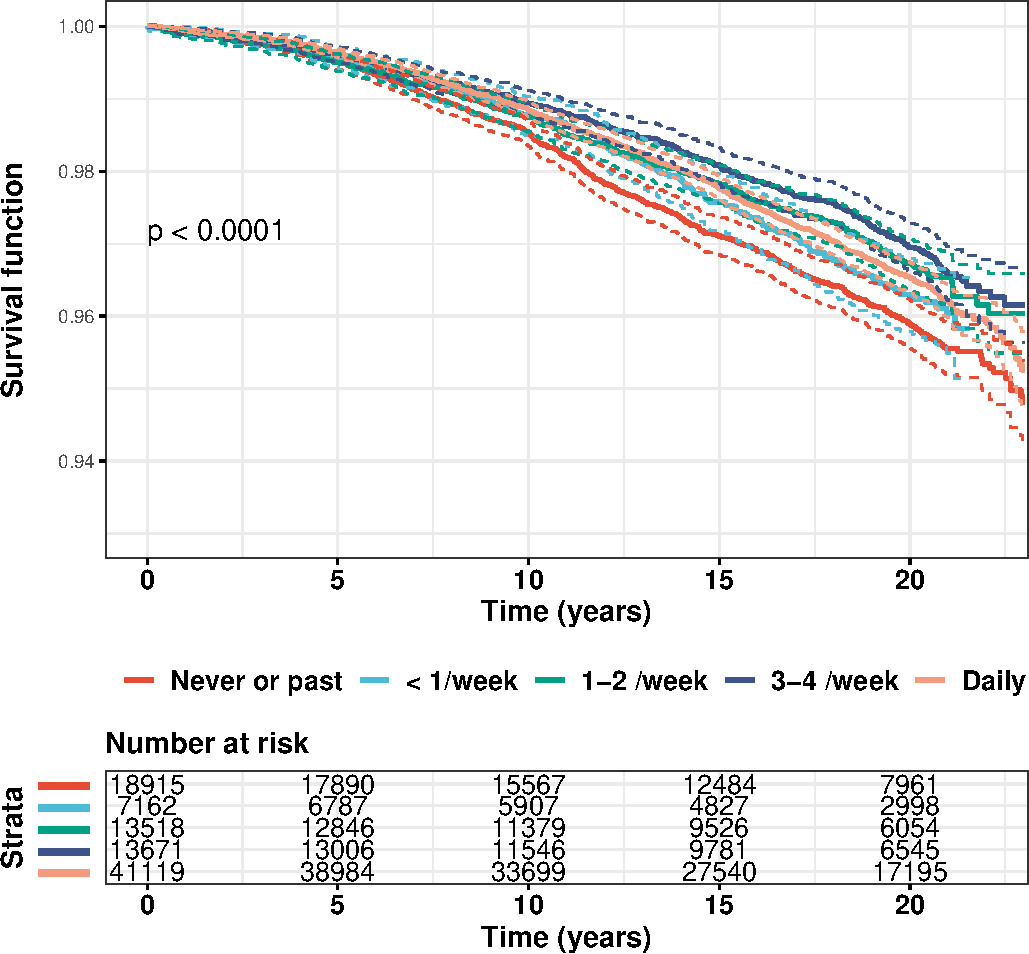
\includegraphics[width=1\linewidth]{traditionalPH_files/figure-latex/fig1-1} 

}

\caption{Kaplan-Meier survival curves for total stroke mortality by drinking frequency (P value was obtained from log-rank tests)}\label{fig:fig1}
\end{figure}

\begin{Shaded}
\begin{Highlighting}[]
\CommentTok{# empty.cox<-coxph(su_obj~1,data=MData)}
\CommentTok{# mgale_res<-resid(empty.cox,type="martingale")}
\CommentTok{# plot(MData$Age,mgale_res, ylim = c(-0.06, 0.01))}
\CommentTok{# lines(lowess(MData$Age,mgale_res)) # not bad}
\CommentTok{# cox1<-coxph(su_obj~ Age,data=MData)}
\CommentTok{# mgale_res<-resid(cox1,type="martingale")}
\CommentTok{# plot(MData$Age,mgale_res, ylim = c(-0.1, 0.01))}
\CommentTok{# }
\CommentTok{# # the relationship seems not linear age should be changed}
\CommentTok{# }
\CommentTok{# }
\CommentTok{# # check the proportional hazard assumption with time }
\CommentTok{# # test for interactions between the explanatory variable and time as below}
\CommentTok{# }
\CommentTok{# age.cox.tt<-coxph(su_obj~Age + tt(Age),data=MData, tt=function(x,t,...) \{x*t\})}
\CommentTok{# summary(age.cox.tt)}
\end{Highlighting}
\end{Shaded}

\end{document}
